\chapter{Некоторые особенности конструкции крейсерско-гоночных яхт}

\section{Классификация и основные требования, предъявляемые к крейсерско-гоночным яхтам}

Яхты для дальних плаваний (крейсерские яхты) можно разделить на три
основные группы, отличающиеся по своему назначению:
крейсерско\-/гоночные, крейсерские и туристские.  Основным назначением
\textbf{крейсерско\-/гоночных} яхт (их правильнее было бы называть
гоночными яхтами открытого моря) является успешное выступление в
маршрутных гонках на длинные дистанции. Крейсерско\-/гоночные яхты
имеют характерное парусное вооружение с узкими и высокими парусами,
свободную палубу, насыщенную механизмами и устройствами для управления
парусами и их настройки (рис.~\ris{32}). Типичными представителями
этой группы яхт являются, например, однотонник <<Марина>>, яхты
<<Конрад-44>> и <<Конрад-54>>.

\begin{figure*}[htb]
  \centering
  \includegraphics[scale=1.3]{0032P}
  \caption{Однотонник <<Марина>> постройки ленинградской судоверфи ВЦСПС}
  \label{fig:32}
  \small
  \centering{}
  1 \--- гребной винт регулируемого шага; 2 \--- перо руля; 3 \--- скоб\-/трап; 4 \--- надувной спасательный плот ПСН-6М; 5 \--- привод натяжного ахтерштага; 6 \--- штурвал; 7 \--- путевой компас; 8 \--- приборная панель; 9 \--- главный компас; 10 \--- двухскоростная лебёдка; 11 \--- односкоростная лебёдка; 12 \--- входной люк; 13 \--- натяжка внутреннего штага; 14 \--- вант\-/путенс; 15 \--- фаловая лебёдка; 16 \--- спинакер\-/гик; 17 \--- натяжка бакштага; 18 \--- вентиляционный дефлектор
\end{figure*}

\textbf{Крейсерские яхты}\index{яхта!крейсерская} \--- достаточно
быстроходные суда, используемые для дальних спортивных плаваний
определённой категории сложности и протяжённости. Суда этого типа
принимают также участие в морских гонках, хотя и с меньшими шансами на
успех при выступлении в одной зачётной группе с гоночными
яхтами. Крейсерские яхты, рассчитанные на многодневное пребывание
экипажа на борту, имеют лучшие условия обитаемости, большие запасы
пресной воды и топлива, часто снабжаются более мощным
двигателем. Такие суда имеют палубные рубки, позволяющие увеличить
объем внутренних помещений и их высоту; конструкцию корпуса,
отвечающую правилам постройки классификационных обществ. При больших
измерениях они оснащаются двухмачтовым вооружением. К судам этой
группы можно, например, отнести однотонник, построенный небольшой
серией на таллинской экспериментальной верфи спортивного судостроения,
яхты типа <<Конрад-45>> и <<Опал>>.

\textbf{Туристские яхты}\index{яхта!туристская} \--- мореходные и
комфортабельные суда, рассчитанные на длительное плавание, не
лимитируемое нормативами времени. Они оснащаются низким парусным
вооружением с относительно небольшой площадью парусности, часто
стилизуются под старинные кечи, шхуны и тендера. Мощный двигатель и
топливные цистерны большой ёмкости позволяют получить высокую скорость
и значительную дальность плавания под двигателем. По скорости и
лавировочным качествам они уступают крейсерским.

В зависимости от мощности двигателя, установленного на яхте, её можно
классифицировать как яхту
\textit{парусно\-/моторную}\index{яхта!парусно-моторная} \--- со
вспомогательным двигателем или как
\textit{моторно\-/парусную}\index{яхта!моторно-парусная}. В первом случае
мощность двигателя составляет 1,5\otdo 2,5~л.с. на каждую тонну
полного водоизмещения яхты, что обеспечивает достижение скорости от 5
до 6 уз. По запасу топлива для двигателя яхта имеет дальность плавания
80\otdo 120 миль; используются гребные винты со складывающимися
лопастями или флюгерного типа, оказывающие минимальное сопротивление
движению яхты под парусами. Двигатель служит лишь для выхода из гавани
и входа в неё, для коротких переходов в штилевых условиях и в
аварийных ситуациях, а также для подзарядки аккумуляторных батарей.

На моторно\-/парусных яхтах удельная мощность двигателя достигает
5\otdo 8~л.с./т.; запасы топлива для него принимаются из расчёта
обеспечения дальности плавания в несколько сотен миль со скоростью
8\otdo 10~уз. Устанавливаются эффективные трёхлопастные гребные винты
большого диаметра, оказывающие на ходу под парусами большое
сопротивление движению. Наличие тяжёлого двигателя и запасов топлива
обусловливает уменьшение массы балласта до 15\otdo 25\,\%
водоизмещения яхты, что, в свою очередь, заставляет ограничивать
площадь парусности. Моторные парусники \--- это туристские яхты, у
которых двигатель является таким же, если не более важным средством
движения, как и паруса.

По району плавания крейсерские яхты делятся на яхты для внутренних
вод, озёрного и прибрежного морского плавания и яхты для открытого
моря (океанские).

\index{яхта!для внутренних вод}
Для плавания по относительно закрытым внутренним водам, характерным
невысокой волной и наличием большого числа пунктов, в которых яхта
может укрыться от непогоды, мореходность яхт может быть ограничена,
корпус, рангоут и такелаж могут иметь лёгкую конструкцию. Оптимальными
типами судов для плавания по внутренним водам являются крейсерские
швертботы, компромиссы, яхты с тяжёлым подъёмным килем и небольшие
килевые суда, осадка которых не превышает 1,4~м. Поскольку при дальних
спортивных плаваниях и гонках такие суда выходят в довольно обширные
водохранилища с неприятной крутой волной, яхты для внутренних вод
следует снабжать самоотливными кокпитами, предусматривать надёжные
закрытия входных и светлых люков и обеспечивать положительную
остойчивость при крене до 90\gr \--- возможность самовыпрямления в
аварийных ситуациях.

Яхты\index{яхта!для озёрного плавания}
\index{яхта!для прибрежного морского плавания},
предназначенные для \textit{прибрежного морского} и
\textit{озёрного плавания}, должны быть рассчитаны на достаточно длительное
противодействие сильному ветру и крупной волне и способность
отлавировать от подветренного берега. Для таких судов обязателен
самоотливной кокпит, прочный рангоут и такелаж, каюта достаточного
объёма, оборудованная койками для отдыха экипажа, работоспособный на
волне камбуз, штурманский стол для ведения прокладки и компас.

Наиболее жёсткие требования к мореходности, оборудованию и снабжению
предъявляются к \textit{яхтам открытого моря}\index{яхта!океанская}.

Для судов, участвующих в гонках, эти требования дифференцируются в
зависимости от сложности маршрута \--- категории гонок.

Самые крупные и мореходные яхты, называемые неофициально яхтами
нулевого класса, или макси\-/яхтами, имеют гоночный балл по правилам
IOR, близкий к максимально допустимому значению 19\otdo 22~м. Такие
суда строятся почти исключительно для трансокеанских и кругосветных
гонок. Они рассчитываются на достижение максимально возможных
скоростей на трассах с попутными ветрами с тем, чтобы ликвидировать
преимущество, которое даёт гандикап меньшим по размерам
яхтам. Наибольшая длина макси\-/яхт составляет 21\otdo 24~м; длина по
КВЛ \--- около 19~м; ширина \--- около 5,5~м; водоизмещение \---
30\otdo 35~т; масса балластного фальшкиля \--- 16\otdo 18~т; осадка
\--- до 3,6~м; обмерная площадь парусности \--- около 240\msq. В
гонках экипаж таких яхт состоит из 13\otdo 17 человек. Корпуса их
строятся из алюминиевых сплавов, реже \--- из стеклопластика или
деревянной конструкции.

Наиболее многочисленную группу яхт на любых гонках составляют яхты
длиной от 10 до 12,5 м (III\--II классов IOR). Среди них имеется
немало сравнительно дешёвых однотипных судов, построенных по одному
проекту что позволяет в ряде случаев выделить их в отдельные стартовые
группы и повысить интерес экипажей к соревнованиям.  Дальнейшим
развитием типизации является введение так называемых <<тонных>> или
<<уровневых>> классов яхт, которые строятся по специальным
правилам. Основным признаком для деления на классы служит величина
гоночного балла IOR. Таких классов шесть: <<двухтонники>> (с гоночным
баллом не более 32 футов \--- 9,76~м); <<однотонники>> (27,5 фута \---
8,38~м); <<3/4-тонники>> (24,5 фута \--- 7,47 м); <<полутонники>>
(21,7 фута \--- 6,60~м); <<четвертьтонники>> (18,5 фута \--- 5,65~м) и
<<минитонники>> (16,5 фута \--- 5,18 м). Для каждого из этих классов
имеются специальные требования к планировке корпуса, оборудованию и
т.\=,п. Это типичные гоночные яхты ограниченной обитаемости, хотя
участвуют в гонках на дистанциях 150\otdo 400 миль. Они могут
выступать и в соревнованиях с яхтами других типов с учётом гандикапа.

Основным требованием, предъявляемым к крейсерско\-/гоночным яхтам,
является их высокая эффективность в гонках при высоких мореходных
качествах.

Высокий надводный борт, большая ширина корпуса и значительная масса
балласта (40\otdo 50\,\%) позволяют обеспечить достаточную
остойчивость яхты для несения эффективной парусности в сильный
ветер. Единственно приемлемым типом вооружения для
крейсерско\-/гоночных яхт малых и средних размеров является бермудский
шлюп благодаря его высоким аэродинамическим качествам. Яхта оснащается
большим числом вспомогательных парусов, средств для их настройки,
позволяющих получить максимальную тягу при ветре любой силы и на любом
курсе яхты по отношению к нему. Работу экипажа с парусами облегчают
палубные шкотовые и фаловые лебёдки, стопора, оттяжки и т.\=,п.

Крейсерско\-/гоночную яхту стараются оборудовать электронными
приборами, облегчающими навигацию и ведение гонки. В их комплект
входят эхолоты, лаги, указатели скорости и направления вымпельного
ветра, курса яхты относительно него, радиопеленгаторы. На крупных и
дорогих яхтах за рубежом не редкость специальные системы
радионавигации <<Декка>>, <<Лоран>> и <<Омега>> и даже аппаратура для
определения места с помощью искусственных спутников Земли. Большинство
яхт снабжаются двумя\-/тремя радиостанциями УКВ и KB диапазонов для
связи с берегом и судейским судном при участии в гонке.

\section{Общее расположение и конструкция корпуса}

Обитаемости крейсерско-гоночных яхт должно уделяться достаточно внимания.

\begin{figure*}[htb]
  \centering
  \includegraphics[scale=1.3]{0033P}
  \caption{Общее расположение однотонника <<Марина>>}
  \label{fig:33}
  \small
  \centering{}
  1 \--- спасательный плот; 2 \--- привод натяжки ахтерштага; 3 \--- кокпит рулевого; 4 \--- колонка штурвала; 5 \--- ахтерлюк; 6 \--- путевой компас; 7 \--- поручень\-/стойка компаса; 8 \--- штурманский стол; 9 \--- кокпит шкотовых; 10 \--- топливный бак; 11 \--- входной люк; 12 \--- стойка лебёдок и стопоров; 13 \--- светлый люк; 14 \--- степс; 15 \--- форлюк; 16 \--- носовой релинг; 17 \--- натяжка штага; 18 \--- паруса; 19 \--- форпик; 20 \--- салон; 21 \--- двигатель; 22 \--- аккумуляторы; 23 \--- конки; 24 \--- моторное отделение; 25 \--- камбуз; 26 \--- шкафы; 27 \--- диван; 28 \--- цистерна питьевой воды; 29 \--- унитаз; 30 \--- стол; 31 \--- умывальник. 
\end{figure*}

Типичным для гоночных яхт является общая компоновка и планировка
внутренних помещений на яхте типа <<Марина>> (см. рис.~\ris{32} и
\ris{33}). Характерной является палуба, свободная от рубок и
надстроек, что диктуется необходимостью обеспечить удобство работы
экипажа с парусами, а также снизить воздушное сопротивление, что важно
при лавировке против сильного ветра. Для того чтобы получить нужную
высоту внутри каюты, корпус яхты выполнен с повышенным бортом и
значительной поперечной прогибью палубы.

Гладкопалубный тип утвердился на яхтах меньших размерений вплоть до
<<минитонников>>. Однако в большинстве случаев для того чтобы
выдержать регламентируемую правилами классов высоту помещения, у входа
устанавливается небольшая рубка, совмещённая с входным люком.

Функционально размещение экипажа в двух кокпитах \--- рулевого в
кормовом у самого транца и шкотовых \--- в кокпите близ
миделя. Располагаясь позади всего экипажа, рулевой контролирует его
действия, имеет хороший обзор парусов, а шкотовые не создают ему
помех. Дифферентовка яхты в меньшей степени зависит от числа людей в
кокпите, так как он находится ближе к общему центру тяжести судна, чем
при традиционном кормовом расположении.

Под палубой экипаж располагается, по существу, в одном большом
помещении в средней части яхты. Поперечная переборка, установленная
под мачтой, отделяет форпик, используемый в качестве парусной
кладовой. Здесь же размещены унитаз с принудительной прокачкой и
небольшая раковина.

Кают\-/компания, она же и каюта для отдыха, оборудована мебелью
облегчённой конструкции и газовым камбузом. Здесь же, близ центра
тяжести яхты, установлен вспомогательный дизель, благодаря чему
существенно снизилось его влияние на период килевой качки и
соответственно уменьшился прирост сопротивления при лавировке против
волны.

В кормовой части судна, отделённой лёгкой полупереборкой, расположена
штурманская каюта со спальными местами для капитана и старшего
помощника. Для оперативной связи штурмана или вахтенного начальника,
ведущего прокладку по карте, с рулевым предусмотрен открывающийся
светлый люк у переднего комингса рулевого кокпита.

Несколько иные принципы планировки общего расположения 15,3\--метровой
яхты, рассчитываемой на длительные гонки и плавания в
океане. Обеспечению комфорта для экипажа в данном случае уделяется
больше внимания. Лёгкими переборками внутренний объем яхты делится на
семь отсеков, или кают. Фор\-- и ахтерпики используются в качестве
шкиперских кладовых. Паруса хранятся в носовом кубрике и в тамбуре
перед мачтой, куда они подаются с палубы через сдвижной люк.

Полная вместимость яхты по числу спальных мест составляет 13 человек,
но трубчатые койки в носовом кубрике и над парусным рундуком
используются только на стоянке и в тихую погоду. Наиболее
комфортабельное помещение \--- кормовая трёхместная каюта (для
владельца или капитана) расположено в непроходной части и через
небольшой лючок сообщается с кокпитом рулевого.

Кают\-/компания, камбуз и штурманская рубка расположены вблизи центра
тяжести яхты, где меньше ощущается килевая качка и удары волн. Здесь
же установлен вспомогательный дизель, закрытый звукоизолирующим
капотом, под пайолами расположены цистерны с запасами топлива и
питьевой воды.

Двухместная каюта в носовой части яхты может быть использована для
размещения вахтенных начальников или гостей.

\begin{figure}[htb]
  \centering
  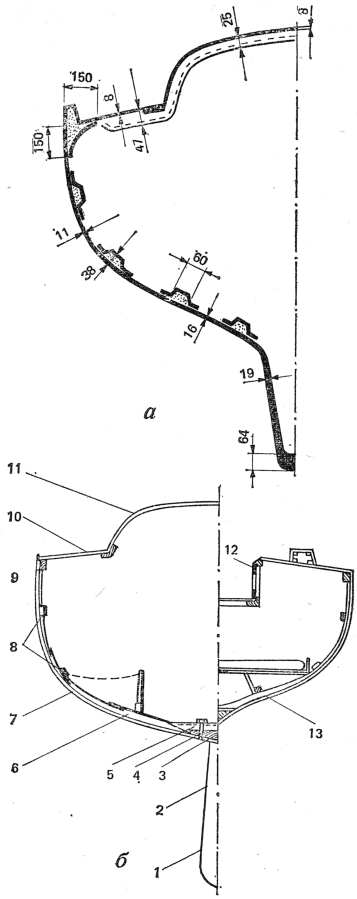
\includegraphics[scale=1.2]{0034P}
  \caption{Конструктивный мидель-шпангоут}
  \label{fig:34}
  \scriptsize
  \centering{}
а \--- пластмассовой яхты длиной 13,2 м; б \--- яхты деревянной конструкции длиной 12,8 м; 

1 \--- внутренний свинцовый балласт 2,73~т; 2 \--- плавник киля, сварной из стальных листов $\delta = 6$~мм; 3 \--- киль $90 \times 460$ мм; 4 \--- болт М25; 5 \--- флор, сталь $\delta = 6$~мм; 6 \--- ламинированный шпангоут $65 \times 125$~мм, клеёный из пяти реек по толщине; 7 \--- обшивка из семи слоев 3-миллиметрового шпона древесины каури (сорт красного дерева); 8 \--- стрингеры $25 \times 50$~мм; 9 \--- привальный брус $50 \times 75$~мм; 10 \--- палуба, три слоя фанеры толщиной по 6,4~мм; 11 \--- рубка, 7 слоев шпона каури $\delta = 3$~мм. 
\end{figure}

Объёмы под койками, шкафы и закрытые полки используются для размещения
личных вещей экипажа и запасов провизии в упаковке.

Освещение и вентиляция внутренних помещений осуществляется через
входной люк и форлюк, снабжённые прозрачными крышками, через
открывающиеся светлые люки на палубе и иллюминаторы в комингсах
рубки. В штормовую погоду помещения вентилируются через дефлекторные
головки типа <<Дорадо>>.

Большую часть внутренних помещений яхты занимают койки, минимальная
длина которых должна быть равна 1950~мм при ширине в голове 650 и в
ногах 500~мм. Каждая койка снабжается закладной доской или парусиновым
обвесом, предотвращающим падение людей при большом крене и качке.

Штурманский уголок оборудуется столом размером не менее
$600 \times 1000$~мм для карт. Около стола или под ним размещаются
ящики для карт, навигационных пособий и прокладочного инструмента. На
переборке закрепляются индикаторы основных навигационных приборов:
лаг, эхолот, указатель курса яхты по отношению к вымпельному ветру,
компас, радиопеленгатор, барометр, часы и т.\=,п. Здесь же может быть
установлена и судовая рация.

Камбуз оборудуется газовой плитой в карданном подвесе, разделочным
столом, мойкой для посуды, ящиками, для расходных запасов провизии,
полками для посуды. Для безопасной работы кока кастрюли должны надёжно
фиксироваться на плите, в удобных местах устанавливают поручни и
подножные упоры, предусматривается откидное сиденье.

Стол в кают\-/компании предпочтителен качающейся конструкции с
противовесами маятникового типа и ограждением для посуды. Стол на
<<Своне-51>> снабжён в средней части глубокими гнёздами для удержания
чашек с бульоном или кофе в штормовых условиях.

Подобная планировка типична для яхт длиной до 18~м и может быть
названа сквозной или проходной, так как все помещения сообщаются между
собой через вырезы в лёгких и прочных поперечных переборках. На более
крупных яхтах применяется отсечный принцип планировки, при которой
некоторые помещения (машинное отделение, форт- и ахтерпики) отделяются
от остальных глухими водонепроницаемыми переборками и имеют
самостоятельное сообщение с верхней палубой.

От конструкции корпуса требуется не только высокая прочность, но и
способность сохранять водонепроницаемость при длительных и многократно
повторяющихся нагрузках.

Корпуса современных яхт строят из качественной древесины,
стеклопластика и лёгких алюминиевых сплавов (реже \--- из стали и
армоцемента). Стеклопластик в настоящее время наиболее
распространённый в мире материал для постройки яхт, особенно малых и
средних (до 16~м длиной) размеров. Благодаря применению методов
холодного формования корпусов в специальных формах \--- матрицах из
стеклопластика возможно изготовить корпус практически с любыми
обводами. В отличие от деревянных и металлических яхт, корпуса которых
собирают из множества деталей набора, обшивки и палубы, корпус
пластмассовой яхты состоит из двух монолитных частей \--- собственно
корпуса и палубы, которая формуется за одно целое с кокпитом и рубкой.

Прочной основой стеклопластика являются несколько слоев
стекловолокнистых материалов. Синтетические смолы, которыми
пропитываются стекломатериалы (на полиэфирной или эпоксидной основе),
при затвердевании связывают слои прочной основы между собой и придают
пластику водонепроницаемость. В наружный отделочный слой смолы
вводится краситель-пигмент, так что при хорошем качестве изготовления
пластмассовый корпус не нуждается в окраске (подводная часть
пластмассовых яхт окрашивается необрастающими красками). В местах,
требующих усиления, при формовании корпуса укладываются дополнительные
слои стекломатериала или заформовываются конструкции из металла.

Жёсткость и прочность корпуса малых пластмассовых яхт обеспечивается
переборками, деталями обстройки каюты, которые приформовываются к
обшивке с помощью <<мокрых угольников>> \--- полос стеклоткани,
пропитанных связующим. Толщина обшивки таких корпусов составляет от 5
до 15~мм. На яхтах длиной более 10~м обшивку дополнительно подкрепляют
продольными стрингерами, выклеиваемыми заодно с обшивкой, или
шпангоутами. Специальные подкрепления в виде флоров и продольных
балок, разносящих нагрузку на большую площадь обшивки,
приформовываются в местах приложения сосредоточенных нагрузок \--- у
степса мачты, в районе крепления балластного фальшкиля, под двигателем
(рис.~\ris{34}, \textit{а}).

Высокая прочность стеклопластика позволяет получить конструкцию
необходимой прочности при малой толщине материала. Однако такая
конструкция, например палуба, не обладает ещё одним важным свойством
\--- жёсткостью, начинает <<дышать>> под нагрузкой. Для повышения
жёсткости палуб, переборок и наружной обшивки часто используют
трёхслойные (сэндвичевые) конструкции. Состоит такая конструкция из
наружных тонких слоев стеклопластика и склеенного с ними внутреннего
слоя \--- заполнителя из прочного лёгкого пенопласта или древесины
бальзы.

Кили на пластмассовых яхтах чаще всего делают в виде сварных
профилированных коробок из нержавеющей стали, которые присоединяют к
корпусу на сквозных болтах, проходящих через усиленные флоры. Иногда
балласт в виде свинцовой или чугунной дроби укладывают в полость киля,
отформованного совместно с корпусом, и заливают связующим, которое
после отвердевания превращается вместе с дробью в монолит.

Корпуса пластмассовых яхт долговечны, легки, стойки к воздействию атмосферы и морской воды, не подвержены гниению и повреждению червями. Недостатком материала является чувствительность к истиранию и к действию концентрированных нагрузок.

Малая жёсткость корпусов требует подкреплять их продольными переборками, как это, например, сделано на яхте <<Конрад-54>>, или трубчатыми ферменными конструкциями для предотвращения общего изгиба корпуса под действием тяги штагов и давления мачты.

В последние годы судостроительная древесина становится все более дефицитным и дорогим материалом на мировом рынке. Для яхтостроения применяются отборная высококачественная древесина тика, красного дерева и сибирского кедра (для обшивки) и дуба (для прочных деталей набора и вообще для всех частей судна), белого и гондурасского кедра. Используются также хорошо выдержанные прямослойная сосна и ель, а также лиственница.

В известной степени выручает широкое применение клеёных конструкций и деталей, в которых можно использовать короткомерный материал. Благодаря качественному подбору древесины в клеёной детали она оказывается более прочной при меньшем сечении. В целом корпус получается более лёгким и прочным, чем собранный на металлическом крепеже.

Клеёной по пазам из реек выполняют и традиционную обшивку вгладь, которая ранее набиралась из досок и конопатилась. Клеёная обшивка монолитная и водонепроницаемая, но имеет; недостаток \--- при сильных колебаниях влажности рейки могут трескаться и усыхать каждая в отдельности. Поэтому для стран с жарким климатом этот метод не применяется. Лучшие яхты строятся с обшивкой из тика в подводной части корпуса и из красного дерева в надводной.

Более лёгкая и прочная \--- двухслойная (а на самых крупных яхтах \--- и трёхслойная) обшивка. Доски внутреннего слоя располагаются диагонально по отношению к ДП, а наружного \--- вдоль судна, поэтому такую обшивку часто называют диагонально\-/продольной. По правилам постройки яхт допускается уменьшение суммарной толщины двухслойной обшивки на 10\,\%, а трёхслойной \--- на 15\,\% по сравнению с монолитной. 

С конца 60-х~гг. получил развитие ещё один метод постройки деревянных корпусов яхт, при котором используются широкие полосы тонкого 3--4\-/миллиметрового шпона, укладываемые диагонально на позитивную форму \--- пуансон в несколько слоев (шпон для постройки лёгких гоночных швертботов и яхт применяется в зарубежной и отечественной практике ещё с 30-х годов). Каждая полоса предварительно пропитывается разжиженным эпоксидным связующим, которое проникает глубоко в поры древесины и консервирует её от загнивания, предотвращает проникновение в обшивку древоточцев. Поверх уложенного и закреплённого временно на пуансоне первого слоя наносится связующее и накладывается второй слой полос и т.д. Эпоксидная смола плотно заполняет все зазоры между кромками полос шпона и объединяет его слои в обшивку-скорлупу, подобную стеклопластиковой. Снаружи корпус может быть покрыт лаком или краской либо оклеен слоем стеклоткани. 

Корпуса небольших яхт по этому методу могут иметь безнаборную скорлупную конструкцию \--- прочность придают детали обстройки интерьера \--- переборки, рундуки и т.\=,п. Более крупные корпуса (самой большой построенной яхтой является 28-метровая копия старинного кэча) формуют прямо по набору, состоящему из редко расставленных переборок и рамных шпангоутов, а также из продольных реечных стрингеров, установленных через 160\otdo 200~мм. По этому же методу делают палубы с надстройками и рубки.

При постройке деревянных корпусов утвердилась поперечная система набора \--- с довольно часто расставленными шпангоутами. Правила постройки яхт регламентируют размеры связей корпуса для различных типов шпангоутов, но наибольшее распространение получила постройка корпуса на гнутых шпангоутах, на ламинированных из реек и на комбинации ламинированных и гнутых. Между парой ламинированных шпангоутов могут устанавливаться два или три гнутых. Для восприятия усилий от фальшкиля и давления мачты в корпусе устанавливают переборки, усиленные рамные шпангоуты (иногда выполняемые из металлических профилей). Внизу ветви шпангоутов соединяют деревянными листовыми или коваными металлическими флорами, разносящими нагрузку на достаточно большую часть шпангоута по ширине корпуса (рис.\ris{34}, \textit{б}).

Палубный настил на деревянных и металлических яхтах делается чаще всего из водостойкой фанеры. Фанерная палуба легче и прочнее обычного настила из палубника \--- не течёт, не рассыхается под воздействием солнца, не требует постоянного ухода. Её можно окрасить, оклеить стеклотканью на эпоксидном связующем или покрыть парусиной на краске. На фанеру могут быть наклеены тонкие декоративные планки из тика, имитирующие традиционный палубный настил. Нелакированная тиковая палуба обладает помимо прочих ещё одним достоинством \--- по ней не так скользко ходить, как по палубе из другой древесины или окрашенной.
 
Корпуса многих крейсерско\-/гоночных яхт, особенно длиной более 15~м, построены цельносварными из алюминиево-магниевых сплавов. Сплавы эти (например, АМг5В) обладают высокой стойкостью против коррозии в морской воде, легко деформируются в холодном состоянии, хорошо свариваются в среде инертного газа аргона. Толщина наружной обшивки на яхтах длиной 15\otdo 16~м составляет 5\otdo 6~мм; килевой пояс может быть изготовлен из листов толщиной до 8~мм. За редким исключением, на алюминиевых яхтах используется поперечная система набора, причём расстояние между шпангоутами составляет 350\otdo 550~мм. Шпангоуты изготовляют из полособульбовых или тавровых прессованных профилей. Свинцовый или чугунный фальшкиль должен быть надёжно изолирован от алюминиевого корпуса с помощью битумной мастики или эпоксидного компаунда.

Крейсерско\-/гоночные яхты из стали в последние годы строят крайне редко, хотя в конце 60-х~гг., когда стальной корпус давал яхте преимущество при обмере по правилам RORC, было построено немало стальных <<однотонников>> и даже яхт меньших размерений. Толщина наружной обшивки на цельносварных яхтах длиной 12\otdo 18~м варьируется от 4 до 6~мм.

Так как сталь и алюминий обладают лучшей теплопроводностью, чем дерево и стеклопластик, на яхтах из этих материалов необходима тепловая изоляция жилых помещений. Такая изоляция в виде плит из экспанзита (прессованная пробка), поропласта и других материалов наклеивается изнутри на наружную обшивку и зашивается декоративными материалами \--- пластиком, фанерой, линкрустом.

Палубы и надстройки металлических яхт изготавливают из фанеры или металла с покрытием деревянным настилом или нескользящей мастикой. 

\section{Устройства, системы и снабжение крейсерско-гоночных яхт}

Безопасность эксплуатации и обитаемость яхты в большой степени зависят от того, насколько хорошо судно оснащено соответствующим оборудованием, устройствами и системами. К числу важнейших судовых устройств относятся якорно\-/швартовное, рулевое, леерное устройства и яхтенный тузик.

\textbf{Якорное устройство.}\index{устройство!якорное}
\index{якорное устройство} Количество и вес становых якорей, калибр якорной цепи и
её длина для крейсерских яхт определяются правилами классификации и
постройки (табл.~\ref{tab:2}). Яхта, уходящая в дальнее плавание,
должна быть укомплектована не менее чем двумя \textit{становыми
якорями}\index{якорь!становой}, один из которых примерно на 20-25\,\%
должен быть тяжелее основного, наиболее часто используемого
якоря. Кроме того, на судне должны быть \textit{завозные
якоря}\index{якорь!завозной} или верпы. Масса самого большого
\textit{верпа}\index{верп} (стоп\-/анкера) принимается обычно равной 75\,\%
основного станового якоря, а самого лёгкого \--- \textit{дрека}\index{дрек}
\--- 25\,\% станового.  Наиболее распространённым типом якоря на
отечественных яхтах остаётся адмиралтейский якорь, обладающий высокой
держащей силой практически на любом грунте. К недостаткам
адмиралтейского якоря относят сравнительно большую массу и
необходимость вооружать его перед каждой постановкой на якорь.

\begin{table*}[htb]
  \centering{}
  \begin{tabular}{p{0.4\textwidth}|c|c|c|c}
    \toprule
    Классы яхты IOR & VI & V & IV~--~II & III \\
    \midrule
    \textbf{Якоря:} \\ 
    количество, шт. &  1 & 1 & 2 & 2 \\
    вес, кг & 15 & 18 & 12, 18 & 18, 25 \\ 
    \midrule
    \textbf{Якорная цепь:} \\
    длина, м & 30 & 30 & 40 & 60 \\
    калибр, мм & 5 & 6 & 7 & 8 \\
    \midrule
    \textbf{Якорный канат:} \\
    окружность, мм & 30 & 50 & 60 \\
    длина, м & 55 & 60 & 70 \\
    \midrule
    \textbf{Завозной канат:} \\
    окружность, мм & 40 & 50 & 60 & 60 \\
    длина, м & 45 & 50 & 55 & 60 \\
    \midrule
    \textbf{Швартовые концы:} \\
    окружность, мм & 45 & 50 & 55 & 60 \\
    длина, м & 5 & 5 & 6 & 8 \\
    \midrule
    \textbf{Ведра}, шт. & 1 & 1 & 1 & 2 \\
    \midrule
    \textbf{Помпа водоотливная} 
    с диаметром цилиндра не менее, мм & 25 & 30 & 40 & 50 \\
    \bottomrule
  \end{tabular}
  \caption{Нормы снабжения крейсерско\-/гоночных яхт якорями, якорными и швартовыми канатами и водоотливными средствами}
  \label{tab:2}
  \textbf{Примечание. }Вес якорей указан для адмиралтейского якоря. При применении бесштоковых якорей их вес должен быть на 25\,\% больше. В случае применения якорей повышенной держащей силы они подбираются по величине держащей силы, которая должна быть не менее, чем у адмиралтейского якоря, указанного в таблице.
\end{table*}

На яхтах находят применение также лёгкие бесштоковые якоря с
поворотными лапами типа Данфорта, Матросова и Холла, а также
якорь\-/плуг (или лемеховый). Относительно своей массы якоря Данфорта,
Матросова и лемеховый развивают очень высокую держащую силу на
песчаных грунтах и в плотном иле, но уступают адмиралтейскому при
стоянке на каменистом грунте и гальке. Кроме того, при съёмке в
сильный ветер, когда яхту без помощи двигателя трудно привести в
положение <<панер>>, требуются большие усилия для отрыва якорей этих
типов от грунта.

Для определения необходимой массы адмиралтейского якоря можно
воспользоваться приближенной формулой:

\begin{equation}
  W = 8 \sqrt[3]{D^2}, \quad \text{кг}
\end{equation}

где $D$ \--- водоизмещение яхты в тоннах. Массу второго якоря можно
принять равной 75\,\% массы первого. Калибр якорной цепи
подсчитывается по формуле:

\begin{equation}
  d = 4,7 \sqrt[3]{D}, \quad \text{мм}
\end{equation}

Якорные цепи предпочтительнее канатов, так как цепь благодаря большой
массе прижимает веретено якоря к грунту и амортизирует рывки яхты при
волнении.

При стоянке на якоре цепь или канат крепятся на яхте за прочный
битенг, кнехт или берётся на стопора. Специальные механизмы для
выборки каната или цепи \--- шпили и брашпили применяются только на
самых крупных яхтах длиной свыше 15~м. Для отрыва якоря от грунта на
яхтах меньших размерений применяют тали со скобой, перекладываемой за
звенья цепи.

Чем ближе к форштевню закреплены клюзы, полуклюзы или роульс для
якорной цепи, тем меньше яхту водит на стоянке и легче выбирается
цепь. Лучшим устройством считается роульс со стопором, установленный
на форштевне.

Для размещения якорных цепей яхты оборудуются цепными
ящиками. Предпочтительнее узкие и высокие ящики, в которые цепь
<<самоукладывается>> без завалов и калышек. Конец цепи крепится на
судне к жвака\-/галсу \--- короткому куску цепи с быстроотдающимся
устройством, которое при полном вытравливании якорь\-/цепи появляется
из палубного клюза и готово к немедленной отдаче.

Необходимым дополнением якорного устройства являются томбуй и буйреп,
а также крепления якорей по\-/походному на их штатных местах.

\textbf{Швартовное устройство}\index{устройство!швартовое} состоит из
битенгов и кнехтов, установленных в носовой и кормовой частях палубы,
киповых планок (полуклюзов), придающих швартовам правильное
направление и предохраняющих их от перетирания о ватервейс или
фальшборт. Длину швартовных концов, для которых используются
синтетические тросы из капрона, лавсана и т.\=,п., рекомендуется
принимать равной удвоенной длине яхты, а диаметр подбирать так, чтобы
разрывная нагрузка троса была бы не меньше водоизмещения яхты.

\begin{figure}
  \centering
  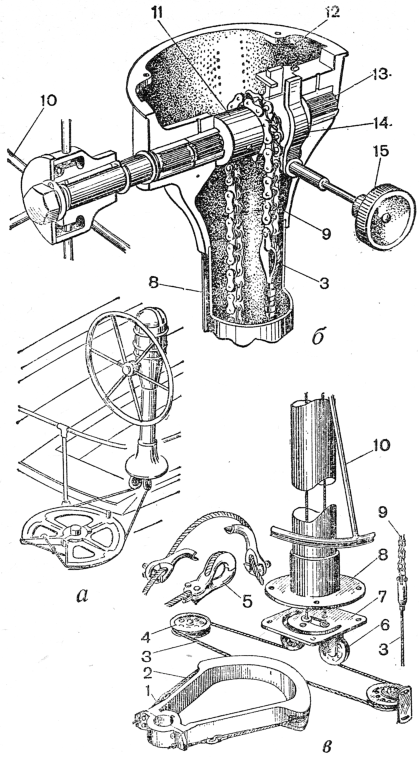
\includegraphics[scale=1.2]{0035P}
  \caption{Рулевой штуртросовый привод со штурвальной колонкой}
  \label{fig:35}
  \small
  \centering{}
  1 \--- натяжное устройство; 2 \--- сектор; 3 \--- штуртрос; 4 \--- направляющий шкив; 5 \--- разъёмный коуш; 6 \--- самоустанавливающийся блок; 7 \--- плита блоков; 8 \--- колонка; 9 \--- цепь Галля; 10 \--- штурвал; 11 \--- звёздочка; 12 \--- корпус рулевой машинки; 13 \--- игольчатый подшипник; 14 \--- колодочный стопор; 15 \--- привод стопора.
\smallskip
\end{figure}

\textbf{Рулевое устройство.}\index{устройство!рулевое} Румпель \---
наиболее простое и надёжное устройство, при котором рулевой хорошо
чувствует яхту, если, конечно, рулевые петли хорошо отцентрированы и
правильно выбран коэффициент компенсации балансирного
руля. Недостатком румпеля являются его длина, мешающая работе в
кокпите, и довольно значительные усилия при управлении яхтой в свежий
ветер. В большую волну при попутных ветрах иногда приходится управлять
яхтой с помощью румпель\-/талей, между румпелем и подходящими утками
на палубе.

Яхты свыше 10~м длиной иногда управляются с помощью штурвала большого
диаметра и тросовой передачи на сектор, закреплённый на баллере над
сальником гельмпорта (рис.~\ris{35}).

Штурвал устанавливается в кокпите на рулевой колонке (\textit{а}) и
имеет на валу звёздочку (\textit{б}), которую огибает роликовая цепь,
включённая в среднюю часть штуртроса. Если на колонке стоит компас, то
детали привода и цепь делаются из немагнитных материалов. Для передачи
применяется гибкий стальной трос конструкции $6 \times 19 +$ос
достаточного диаметра, чтобы выдержать рывки, передаваемые рулём на
волнении. Критическое значение имеют диаметры направляющих шкивов и их
ориентация точно по оси троса; диаметр шкива по желобку для троса
должен быть не менее 16\otdo 19 диаметров троса.

Штуртросовый привод не является самотормозящимся в отличие от ранее
применявшихся винтовых рулевых машинок, поэтому рулевой сохраняет (при
отсутствии люфтов) хорошее чувство руля. Тормоз, имеющийся на колонке,
позволяет застопорить руль в определённом положении и на
стоянке. Сектор (\textit{в}) (иногда он заменяется диском с желобками
для троса) снабжается тросовыми или другими ограничителями поворота
руля.
 
\textbf{Леерное устройство}\index{устройство!леерное} состоит из
жёстких трубчатых ограждений \--- релингов, установленных в носу и
корме, стоек и лееров. Размеры и конструкция леерного ограждения
регламентируются правилами обеспечения безопасности плавания при
проведении крейсерских гонок.

Для того чтобы большой генуэзский и стаксель не ложился на леера,
носовой релинг выполняют разрезной конструкции \--- со щелью, в
которую проходит нижняя шкаторина генуи на острых курсах. На леерах в
районе кокпита закрепляют парусиновые обвесы, защищающие экипаж от
ветра и брызг. С внутренней стороны на них пришивают карманы для
бросательного конца и других мелких предметов снабжения, которые
желательно иметь на палубе.

На яхте, выходящей в крейсерское плавание, \textbf{тузик}\index{тузик}
является необходимой деталью снабжения. Минимальные размеры тузика,
позволяющие безопасно использовать его на закрытых акваториях: длина
\--- 2,4~м, ширина \--- 1,2~м, высота борта \---
0,4~м. Предпочтительнее тузики с катамаранными обводами или с носовым
транцем, как более вместительные и остойчивые на
волнении. Существенными деталями оборудования тузика являются мягкий
круговой кранец, закреплённый по привальному брусу, рым для буксировки
в нижней части форштевня или на киле, гнездо в транце для голанения и
подвески якоря при его завозе. На палубе яхты или на крыше рубки
предусматривают подушки для укладки тузика и обушки для крепления
найтовов. Для подъёма шлюпки массой более 100~кг на палубу
используются гик, специальная стрела или шлюпбалки.

\textbf{Системы.} Крейсерско\-/гоночные яхты оборудуются осушительной,
сточной, вентиляционной системами, а также системами водо- и
газоснабжения.

\textit{Осушительная система}\index{система!осущительная} состоит из ручных
насосов, приёмных трубопроводов с сетками и отливных трубопроводов,
выведенных за борт выше ватерлинии. Применяются ручные диафрагменные
помпы, одно- и двухцилиндровые насосы, а также
насосы-альвееры. Правила классификации оговаривают производительность
насоса или Диаметр его цилиндра (см. табл.~\ref{tab:2}). Диаметр
трубопроводов составляет обычно половину диаметра цилиндра.

Согласно правилам безопасности крейсерских гонок, на яхтах,
участвующих в гонках 1--3-й категорий, одна из помп обязательно должна
быть установлена так, чтобы ею можно было пользоваться из кокпита,
когда все входные люки закрыты. Простейший вариант \--- всасывающая
поршневая помпа, смонтированная в днище кокпита, в который она подаёт
трюмную воду, сливающуюся самотёком через отливные шпигаты.

Если отливной трубопровод выводится за борт, он должен быть снабжён
невозвратно\-/запорным клапаном.

К приёмнику осушительного насоса должен быть обеспечен
беспрепятственный сток воды через все флоры и переборки либо к
распределительному коллектору у помпы из каждого отсека подводятся
отдельные трубопроводы.

\textit{Система водоснабжения}\index{система!водоснабжения} на яхте
состоит из цистерн пресной воды (они обычно размещаются под пайолами
вблизи центра тяжести яхты), наливных и воздушных труб, расходных
трубопроводов с насосом и кранами.

Цистерны большой ёмкости снабжают продольными отбойными
переборками. Наливная труба заканчивается на палубе герметичной
резьбовой пробкой, а конец воздушной трубки располагается так, чтобы
исключить попадание внутрь цистерны морской воды и быть на виду при
заполнении цистерн.

На яхтах получили распространение две системы подачи воды из цистерн к
раковинам на камбузе и в умывальнике:
\textit{гравитационная}\index{система!водоснабжения!гравитационная} \---
самотёком из небольшой расходной цистерны, располагаемой под палубой,
или под давлением воздуха, которое создаётся при нагнетании воды в
полузаполненную расходную цистерну (гидрофор)
(рис.~\ris{36}). \textit{Гидрофор}\index{система!водоснабжения!гидрофорная}
располагается под пайолами и не занимает полезного объёма внутри
яхты. В обоих случаях насос пресной воды может быть ручным или с
электроприводом от аккумуляторной батареи. Вода на камбуз может
подаваться с помощью ручной или педальной диафрагменной помпы
непосредственно к расходному крану.

\begin{figure}[htb]
  \centering
  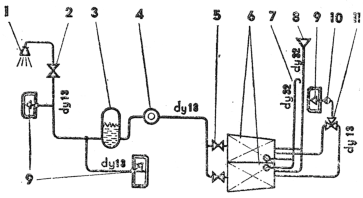
\includegraphics[scale=2]{0036P}
  \caption{Схема системы водоснабжения с гидрофором (под давлением)}
  \label{fig:36}
  \small
  \centering{}
  1 \--- душ; 2 \--- запорный кран \textit{dу} 13; 3 \--- гидрофор ёмкостью 30 литров; 4 \--- нагнетательный насос; 5 \--- запорный кран \textit{dy} 18; 6 \--- цистерны пресной воды; 7 \--- воздушная трубка; 8 \--- заливная горловина; 9 \--- раковина; 10 \--- педальная диафрагменная помпа; 11 \--- трёхходовый кран \textit{dy} 13

  (\textit{dy} \--- внутренний диаметр трубопровода)
\end{figure}

Постоянно повышающиеся требования к чистоте водной среды не оставляют
в стороне и спортивные суда. В настоящее время на многих яхтах
устанавливают специальную сточную систему, содержащую цистерну, в
которой собираются загрязнённые воды от камбуза, умывальника и
гальюна. Опорожнение этой цистерны производится с помощью специальных
установок в гаванях. Непосредственный выброс сточных вод за борт
допускается во многих районах моря только за пределами трёхмильной
прибрежной зоны.

Унитазы на яхтах, как правило, оказываются расположенными ниже
ватерлинии, вследствие чего необходимо специальное устройство для
промывки забортной водой и откачки грязной воды за борт, если судно не
оборудовано сточной цистерной.

На многих яхтах используются \textit{газовые камбузные
  плиты}\index{система!камбуз}. При значительном числе экипажа и
автономности плавания требуется установка баллонов большой ёмкости и
монтаж системы газоснабжения.

Пропан\-/бутан тяжелее воздуха, оказывает отравляющее действие на
организм человека, и смесь его с воздухом в определённой пропорции
взрывоопасна. Поэтому к системе газоснабжения предъявляются особые
требования. Баллоны с газом должны устанавливаться в вертикальном
положении, желательно в помещении, изолированном от жилых кают или на
верхней палубе. Дно помещения для баллонов должно располагаться выше
ватерлинии и иметь шпигат для стока газа за борт. Отсек баллонов
должен хорошо вентилироваться.

Газовые баллоны снабжаются редукционными клапанами для понижения
давления с 8\otdo 16~атм до 0,05~атм. Трубопровод, соединяющий баллон
с плитой, выполняется из медных труб или дюритового шланга с
минимальным количеством соединений и с запорным краном перед плитой.

\begin{figure}[htb]
  \centering
  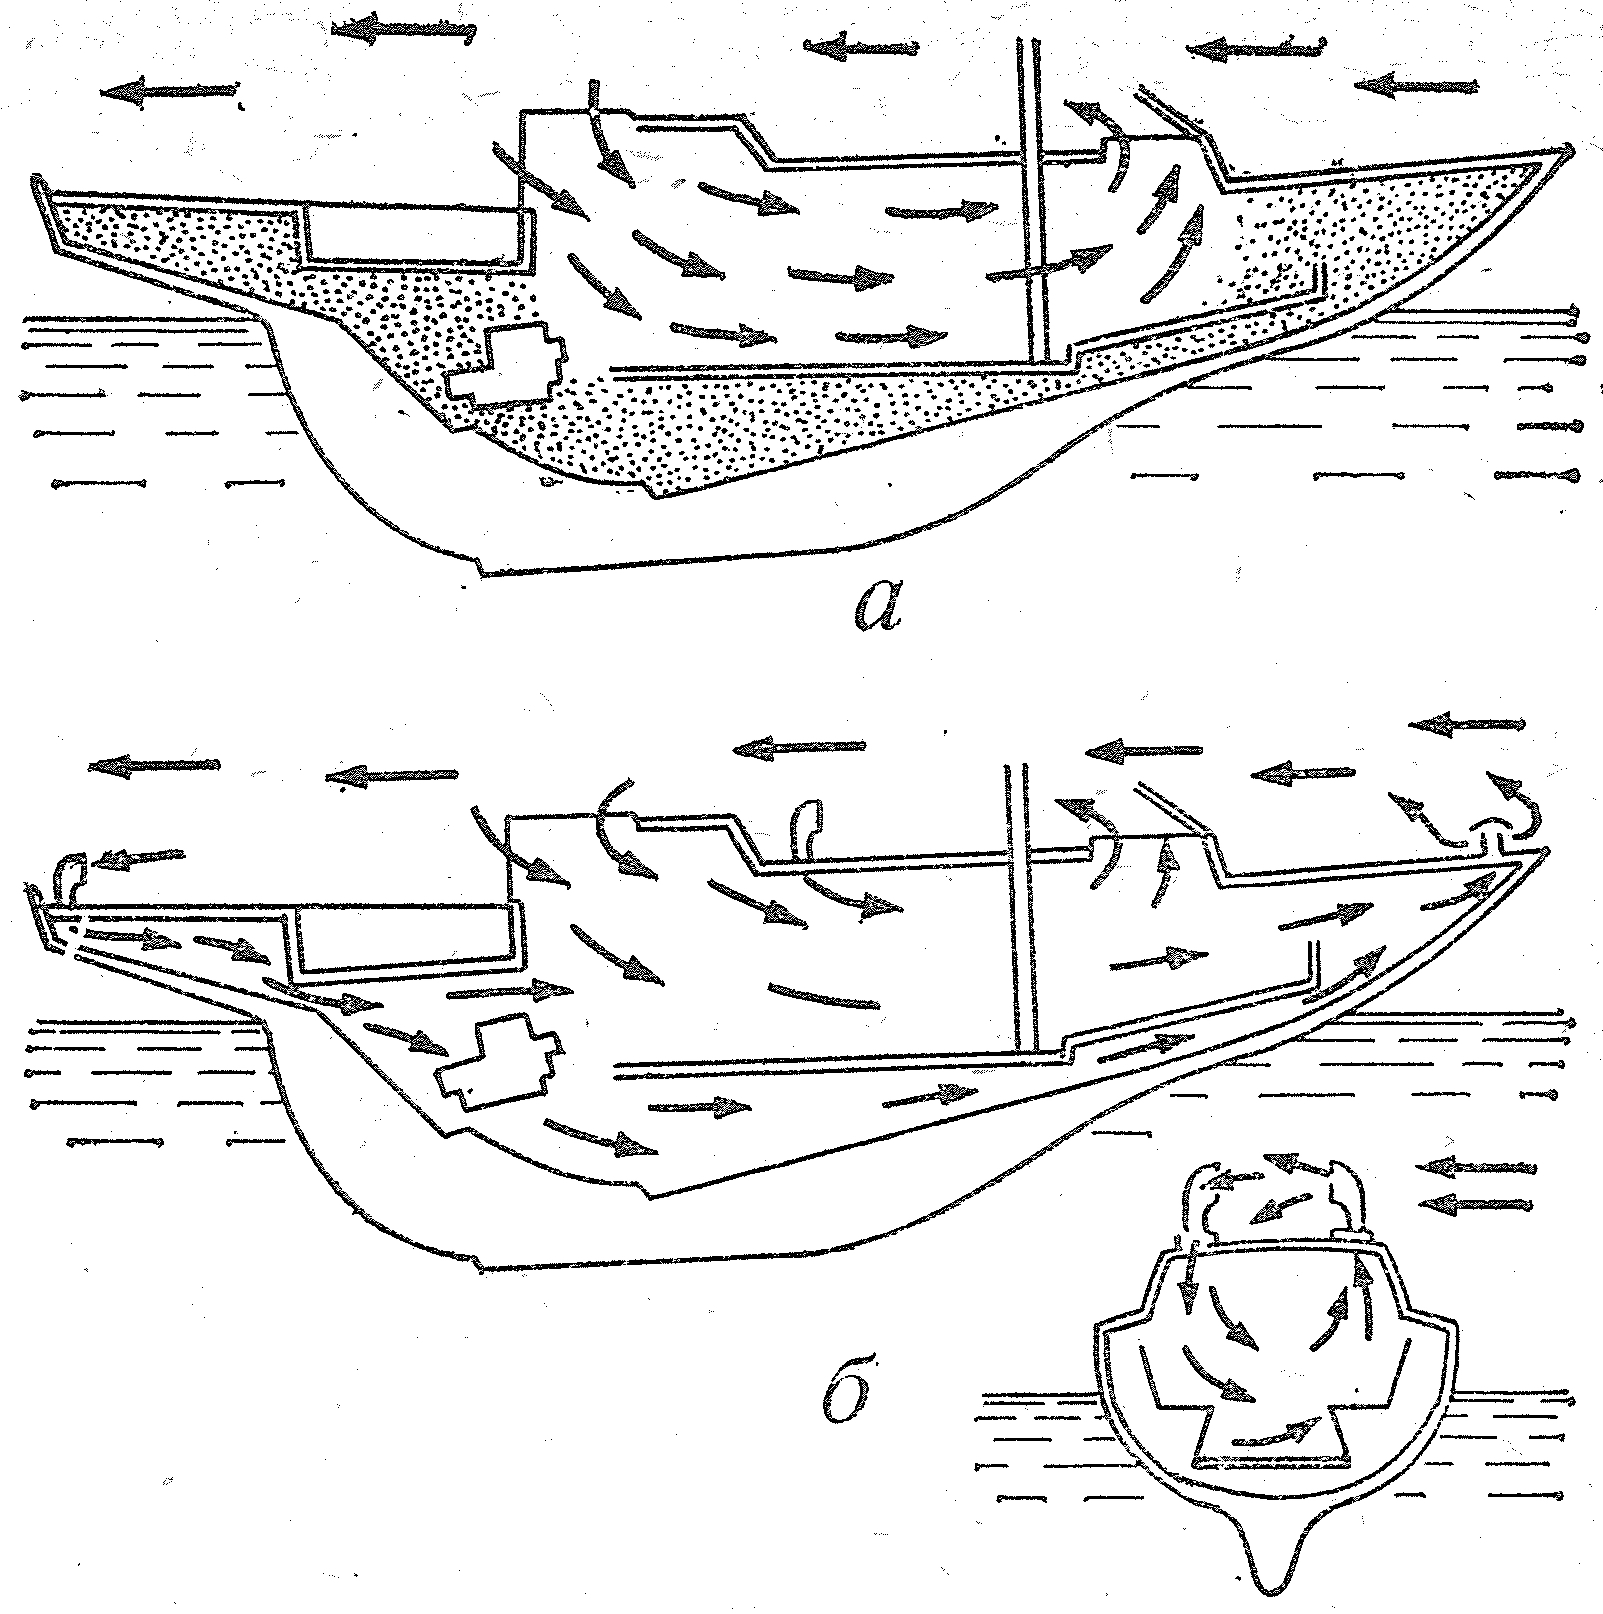
\includegraphics[scale=1.2]{0037P}
  \caption{Схема циркуляции воздуха в помещениях яхты}
  \label{fig:37}
  \small
  \centering{}
  \textit{а} \--- недостаточная циркуляция воздуха (заштрихованы невентилируемые объёмы); \textit{б} \--- правильная циркуляция воздуха
\end{figure}

\textit{Система естественной вентиляции}\index{система!вентиляции!естественная}
должна обеспечивать непрерывную циркуляцию воздуха во всех помещениях
яхты (рис.\ris{37}). Это возможно, если расположить нагнетательные
вентиляционные головки в корме, а поток воздуха в помещениях судна
направить с кормы в нос. Хорошая вентиляция важна не только для
нормальных условий жизни экипажа в море, но и для увеличения срока
службы самой яхты. При плохой вентиляции (особенно трюма и
пространства между наружной и внутренней обшивками) на деревянных
деталях корпуса появляется грибковая плесень и гниль.

Наиболее распространённые тип вентиляционных головок, используемые как
для притока, так и вытяжки представлены на рис.~\ris{38}.

\begin{figure}[htb]
  \centering
  \includegraphics[scale=1.2]{0038P}
  \caption{Вентиляционные головки брызгозащищенного типа для яхт}
  \label{fig:38}
  \small
  \centering{}
  \textit{а} \--- типа <<Дорадо>>; \textit{б} \--- фирмы <<Никро Фико>>
\end{figure}

При установке вспомогательного двигателя моторный отсек отделяется от
остального трюма водонепроницаемым флором или переборкой. Под
двигатель устанавливают поддон для сбора утечек топлива и
масла. Топливные баки располагают по возможности (бензобаки \---
обязательно) вне моторного отсека, а горловины для их заполнения и
воздушные трубки выводят на палубу.

Двигатели обслуживаются системами: топливной, водяного охлаждения,
газовыхлопной.

\textbf{Электрооборудование.}\index{электрооборудование} Для
внутреннего освещения кают и питания навигационных огней применяется
постоянный ток напряжением 6\otdo 12~в на малых яхтах и 24~в \--- на
больших. Источниками тока служат кислотные или щелочные аккумуляторные
батареи, которые подзаряжаются от генератора, навешенного на
двигатель, или через зарядное устройство от береговой сети. Ёмкость
батареи составляет обычно 100\otdo 300~а-ч.

Мощность ламп для внутреннего освещения кают достаточна 15\otdo 25~вт,
Для навигационных огней и освещения палубы \--- 12\otdo 15
вт. \textit{Отличительные бортовые огни}\index{огни!отличительные}
устанавливают на носовом релинге, на комингсах рубки или на краспицах
таким образом, чтобы их не закрывали паруса. \textit{Белый
топовый огонь}\index{огни!топовый, белый}, который яхта должна нести
при движении под мотором, устанавливается на передней мачте на высоте
2\otdo 5~м над палубой, а \textit{кормовой}\index{огни!кормовой} \--- на
кормовом релинге или гакаборте\footnote{На яхте --- край палубы на
  корме у транца, ограниченный его шириной.}. В качестве \textit{якорного
штагового огня}\index{огни!якорный}\index{огни!штаговый} можно
использовать переносную лампу; для сигнализации служит \textit{клотиковый
огонь}\index{огни!клотиковый}, устанавливаемый на топе мачты. Яхты
внутреннего плавания должны быть снабжены импульсными
лампами\-/отмашками, расположенными на вантах или комингсах рубки.

Для освещения палубы и парусов на нижних краспицах устанавливают фары
мощностью 6\otdo 12~вт. Для освещения компаса, штурманского стола и
камбуза предусматривается автономное освещение.

Аккумуляторы устанавливают в моторном отделении вблизи стартера
двигателя и заключают в водонепроницаемые ящики с вентиляционными
трубками. Электропроводка выполняется морским кабелем. Потребители
электроэнергии разбиваются на несколько групп, каждая из которых
снабжается на распределительном щите отдельными предохранителями и
выключателями.

\section{Парусное вооружение}

Подавляющее большинство крейсерско\-/гоночных яхт, принимающих участие
в гонках, оснащается \textbf{одномачтовым вооружением типа
шлюп}\index{шлюп}\index{парус!вооружение!шлюп} даже при площади
парусности 150\otdo 200\msq. Шлюп обладает высокими тяговыми
характеристиками, прост в управлении и обеспечивает хорошую
управляемость яхты.

Однако при увеличении парусности свыше 100\msq становятся ощутимы
недостатки оснастки этого типа, которые требуют подчас сложных
конструктивных решений. Увеличивается высота мачты и соответственно
размеры её поперечного сечения и масса: для раскрепления мачты
требуется тяжёлый стоячий такелаж. Высокое расположение центра
парусности вызывает необходимость повышать остойчивость, увеличивать
массу балласта. При усилении ветра экипажу приходится брать рифы на
гроте и заменять передние паруса на меньшие по площади. В прошлом при
парусности 60\otdo 200\msq яхты нередко оснащались \textbf{вооружением типа
иол}\index{иол}\index{парус!вооружение!иол}. Площадь бизани на иоле
составляет всего 10\otdo 12\,\% общей площади парусности, и роль этого
паруса в создании тяги невелика. Бизань, однако, оказывает
существенное влияние на центровку яхты, обеспечивает исключительную
поворотливость, особенно когда в штормовых условиях несут небольшой
стаксель в комбинации с бизанью.

\textbf{Вооружение типа кэч}\index{кэч}\index{парус!вооружение!кэч}, которое
целесообразно при оснащении яхт парусностью 120\otdo 250\msq благодаря
более равномерному распределению общей площади между тремя основными
парусами (бизань \-- 20\otdo 25\,\%, грот \--- 45\otdo 50\,\%,
стаксель \--- 30\otdo 35\,\%) предпочитается для оснащения крейсерских
и гоночных океанских макси\-/яхт. Для уменьшения влияния стекающего с
грота потока воздуха на работу бизани бизань\-/мачту часто относят на
значительно большее расстояние от грот\-/мачты, чем при традиционной
оснастке этого типа.

Кэч обладает заметно худшими качествами на лавировке, чем шлюп или
иол, но лучше идёт под стакселем и бизанью и устойчивее лежит в
дрейфе, чем иол.

\textbf{Тендер}\index{тендер}\index{парус!вооружение!тендер} в его классическом
виде \--- с двумя или тремя передними парусами \--- стакселем и
кливером, так же как и
\textbf{шхуна}\index{шхуна}\index{парус!вооружение!шхуна}, в последние годы
практически не применяется. Многие шлюпы снабжаются внутренним
(нижним) штагом, на котором могут ставиться дополнительные стаксели
как в слабые, так и в свежие ветра. Но основную роль играет топовый
генуэзский стаксель. Шхуной вооружают яхты парусностью 200\otdo
300\msq, причём используется преимущественно стаксельное вооружение.

В 60-е~гг. крейсерско\-/гоночные яхты предпочитали \textbf{вооружать шлюпом с
топовым стакселем} \index{шлюп!с топовым стакселем}\index{парус!вооружение!шлюп!с топовым стакселем},
поскольку стаксель является более эффективным парусом, чем грот. К
тому же при топовой оснастке допускается постановка спинакера большей
площади, чем при оснастке типа $7/8$ или $3/4$ \--- по положению точки
крепления основного штага относительно общей высоты мачты. В последние
годы, однако, наметилась тенденция вновь оснащать яхты, особенно
младших классов (четверть- и полутонники) \textbf{шлюпом типа
$7/8$}\index{шлюп!$7/8$}\index{парус!вооружение!шлюп!$7/8$} или
$3/4$\index{шлюп!$3/4$}\index{парус!вооружение!шлюп!$3/4$}. Как
показал опыт параллельных испытаний однотипных яхт, топовый и $7/8$
варианты равноценны по лавировочным качествам. На полных курсах яхта с
топовой оснасткой получает преимущество в скорости благодаря большей
площади спинакера. Однако уже на крутом бакштаге из-за малой площади
грота топовый шлюп проявляет склонность к брочингу. На бакштаге и
галфвинде шлюп типа легче в управлении как благодаря меньшей величине
сил, действующих на спинакере, так и за счёт повышения роли грота.

К достоинствам оснастки типа $7/8$ относят также меньшее сечение мачты и
возможность регулировать её изгиб с помощью штагов и бакштагов. Этот
тип оснастки лучше для сильных и свежих ветров; топовая оснастка
предпочтительна для слабого ветра.

Подавляющее большинство яхт оснащается мачтами, изготовленными методом
прессования из алюминиево-магниевых сплавов. Оптимальные весовые
характеристики получаются в случае использования профилей мачты с
переменной толщиной стенки, утолщающейся в тех местах поперечного
сечения, где действуют наибольшие напряжения
(рис.~\ris{39}). Соотношение размеров продольной и поперечной оси
сечения составляет 1,25\otdo 1,50. Для яхт меньших размерений
применяются мачты овального сечения и с постоянной толщиной стенки.

Деревянные мачты выполняются клеёной пустотелой конструкции овального
или прямоугольного сечения со скруглёнными углами. Толщина стенок
составляет 1/5 поперечного размера, а в местах крепления такелажа и в
нижней части мачта делается сплошной.

Алюминиевые мачты на 40\,\% легче деревянных и более надёжны в
длительной эксплуатации и позволяют сделать внутреннюю проводку фалов,
чем существенно снизить воздушное сопротивление.

\begin{figure}[htb]
  \centering{}
  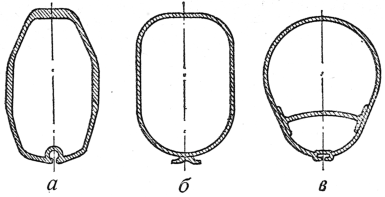
\includegraphics[scale=1.2]{0039P}
  \caption{Поперечное сечение мачт из лёгкого сплава}
  \label{fig:39}
  \centering{}
  \small
  \textit{а} \--- мачта с переменной толщиной стенки для топовой оснастки крупных яхт; \textit{б} \--- мачта крейсерской яхты водоизмещением около 3~т; \textit{в} \--- мачта мореходной крейсерско\-/гоночной яхты
\end{figure}

\textit{Стоячий такелаж}\index{стоячий такелаж}\index{такелаж!стоячий}
изготавливается из жёстких стальных тросов конструкции
$1 \times 19$ \--- спиральной свивки из 19 нержавеющих стальных
проволок. В отечественной практике применяется трос
$6 \times 7 + $\,1ОС, а на зарубежных яхтах можно видеть такелаж из
сплошной нержавеющей проволоки. Следует помнить, что от жёсткости
троса зависит распределение нагрузки от парусов между мачтой и стоячим
такелажем. Чем меньше проволок в пряди при данном диаметре троса, тем
больше его жёсткость и тем на меньшую длину он растягивается при
повышении нагрузки \--- усилении ветра. Особенно важно иметь жёсткий
трос на стоячем такелаже в верхней части мачты \--- на топ\-/вантах,
штаге и ахтерштаге с тем, чтобы уменьшить его прогиб, который
увеличивается по мере удаления от опорной точки \--- пяртнерса или
степса.

Суммарная разрывная нагрузка, которую должны выдерживать ванты одного
борта, составляет около $1,25D$ \--- водоизмещения яхты. Это
показатель не только прочности, но и жёсткости стоячего
такелажа. Между отдельными вантами суммарную нагрузку можно
распределить в зависимости от схемы раскрепления мачты такелажем, и в
первую очередь от количества краспиц (рис.~\ris{40}).

Для штага и ахтерштага при топовом стакселе применяют такой же трос,
как и для самых прочных вант. Следует учитывать, что обрыв штага
равносилен потере мачты. При оснастке типа 7/8 штаг должен иметь такую
же прочность, что и одиночные нижние ванты; ахтерштаг и бакштаги \---
не менее прочности троса для верхних вант.

\begin{figure}[htb]
  \centering{}
  \includegraphics[scale=1.2]{0040P}
  \caption{Схема раскрепления мачт крейсерско-гоночных яхт и нагрузки на ванты в процентах от общего усилия}
  \label{fig:40}
\end{figure}

Важное значение имеет угол между мачтой и вантой. Угол менее 12\gr
можно считать недостаточным \--- получается большое усилие сжатия в
мачте, а ванты необходимо вырубать из более толстого троса. Оснастка с
тремя парами краспиц позволяет увеличить угол между вантами и мачтой в
полтора раза. Длина нижних краспиц при трёх рядах краспиц может быть
увеличена, так как ближе к палубе <<пузо>> генуи увеличивается и она
не касается концов краспиц.

Стоячий такелаж яхты является инструментом для настройки грота и
оказывает влияние на работу стакселя. Если на малых яхтах (швертботах)
в слабый ветер при прогибе топа мачты на подветренную сторону нагрузка
на грот и крен яхты уменьшается, то на больших судах это
недопустимо. Отклонившийся от среднего положения топ означает
уменьшение угла между мачтой и вантой, снижение поддерживающей
способности ванты, увеличение прогиба штага. Кроме того, увеличивается
плечо приводящего к ветру момента.

Поэтому на яхтах с топовым вооружением важно установить топ мачты
жёстко и точно в \textit{ДП} и не допускать его отклонения под
нагрузкой. При установке мачты её выравнивают с помощью клиньев в
пяртнерсе строго по \textit{ДП}. Затем, подняв на грота\-/фале
рулетку, регулируют положение топа с помощью натяжения верхних вант,
контролируя по рулетке равные расстояния от топа до симметричных
относительно \textit{ДП} точек на правом и левом фальшбортах. Затем
добиваются с помощью натяжения средних и нижних вант прямолинейности
ликпаза по всей высоте мачты.

Верхние ванты набивают так, чтобы на ходу в средний ветер при крене
15\otdo 20\gr подветренная ванта была бы не слишком туго набита, не
имела бы слабины. Натяжение средних и нижних вант делается несколько
меньше. Если нижние ванты двойные, то сначала набивают передние, с тем
чтобы они были несколько более тугими.

Необходимое натяжение придаётся штагу обычно с помощью ахтерштага при
топовом вооружении и бакштагов при оснастке типа 7/8. Ахтерштаг
выбирается так туго, как только это возможно: предварительное его
натяжение может составлять 30\otdo 40\,\% разрывной нагрузки троса.

Используя продольный такелаж, экипаж крейсерско\-/гоночной яхты имеет
возможность регулировать изгиб мачты в продольной плоскости и тем
самым изменять профиль грота в зависимости от ветровых условий. Для
придания мачте прогиба применяют два основных способа: с помощью
перемещения мачты в пяртнерсе вперёд и с помощью натяжения ахтерштага
при слегка ослабленном штаге. Величина прогиба мачты невелика: в
зависимости от размеров поперечного сечения мачты, схемы оснастки,
устройства краспиц и т.\=,п. она может составлять от 1/2 до 3/4
продольного размера поперечного сечения мачты. Однако и этого
достаточно, чтобы сделать грот более плоским при усилении
ветра. Величина прогиба регулируется с помощью внутреннего штага и
бакштага. Нижний конец этого штага снабжается ползуном, скользящим по
продольному рельсу, и мощными талями, позволяющими создать достаточное
натяжение штага. При перемене галса внутренний штаг приходится
отдавать для переноса генуи на другой борт.

С помощью продольного такелажа можно изменять в довольно широких
пределах наклон мачты с целью получения оптимальной центровки яхты.

Управление наклоном мачты осуществляется с помощью гидроцилиндров на
фор- и ахтерштагах, связанных трубопроводами в общую систему, либо
механически с помощью винтовой натяжки и <<бесконечного>> троса,
соединяющего штаги под палубой. Величина перемещения топа на крупных
яхтах может достигать 1,2\otdo 1,5~м.

Паруса крейсерско\-/гоночных яхт шьются из синтетических тканых
материалов на основе волокон полистера \-- продукта крекинга
нефти. Впервые такая ткань под названием терилен была сделана в
1941~г. в Англии, а применение её для парусов началось с
1951~г. Аналогичные материалы, изготавливаемые в других странах,
получили другие названия: дакрон (в США), лавсан (в СССР), тергал (во
Франции), тревира (ФРГ) и т.\=,п. Это лёгкие и прочные ткани,
обладающие необходимой плотностью и гладкостью поверхности. Последние
два свойства достигаются каландрованием и в ряде случаев пропиткой в
небольших количествах синтетической смолой.

Благодаря заполнению смолой микропор между нитями ткани уменьшается её
склонность к повышенной деформации при действии растягивающей нагрузки
по диагонали \--- под углом к нитям основы и утка, что приводит к
большим искажениям формы паруса. Синтетика не гниёт, устойчива к
воздействию масел и многих химических веществ.

Хлопчатобумажная парусина \--- миткаль и перкаль, из которых иногда
ещё шьют паруса, существенно уступают дакрону и лавсану по прочности,
воздухонепроницаемости, а главное \--- паруса из них под нагрузкой
получают большую остаточную деформацию \--- вытягиваются.

Лёгкие спинакеры шьют из нейлона \--- ткани на основе полиамидного
синтетического волокна, получаемого из каменного угля. Эта ткань
сильно тянется под нагрузкой, хотя остаточные деформации парусов
невелики, и недостаточно стойкая к воздействию солнечных лучей.

При выборе ткани для парусов кроме её прочности следует учитывать ещё
и фактор деформации под нагрузкой. Паруса из лёгкой ткани, конечно,
более удобны для укладки и хранения, однако в сильный ветер они сильно
вытягиваются и теряют свою форму.

<<Пузо>> паруса перемещается назад, он становится
малоэффективным. Помимо размеров и площади парусов играют роль также
размерения яхты, её водоизмещение и район плавания. Для парусов яхт
открытого моря используется ткань более тяжёлая, чем для яхт,
плавающих на внутренних воде хранилищах и в закрытых
заливах. Приближённо вес ткани (дакрон или лавсан) для основных
парусов можно рассчитать по формуле:

\begin{equation}
  \omega = 33 \cdot \lkvl \, ,
\end{equation}

где $\omega$ \--- вес ткани,\gmsq; \lkvl \--- длина яхты по КВЛ, м.

Таким образом, для яхт длиной по ватерлинии 9\otdo 10~м для грота и
стакселя необходима ткань весом 300\otdo 340\gmsq. Генуэзские стакселя
на таки яхтах шьют из ткани весом 245\otdo 400\gmsq; лёгкую геную \---
из ткани 130\otdo 200\gmsq; для спинакеров используется нейлон весом
около 100\gmsq.

Для того чтобы пройти дистанцию гонки с максимально возможной
скоростью, яхта должна быть оснащена достаточным числом сменных
передних парусов, рассчитанных на плавание различными курсами по
отношению к ветру, скорость которого может изменяться в течение
гонки. Правила обмера ІOR в целях снижения стоимости оснащения яхт для
гонок ограничивают число парусов, которое может быть на борту судна во
время соревнований. Кроме основного грот разрешается иметь запасной,
сшитый из той же ткани, что и основной, один штормовой комплект из
трисель и стакселя. Количество стакселей спинакеров ограничивается для
каждого класса. На иолах и кечах можно иметь ещё запасную бизань и три
бизань\-/стакселя (апселя).
 
\begin{figure}[htb]
  \centering{}
  \includegraphics[scale=1.2]{0041P}
  \caption{Типичное оснащение крейсерско-гоночной яхты парусами}
  \label{fig:41}
\end{figure}

Передние паруса являются основным движителем яхты, поэтому и подбору
уделяется много внимания. Характерный для топовой оснастки небольшой
яхты ($\lkvl \approx 8$~м) набор парусов представлен на рис.~\ris{41}.

\textbf{Дрифтер}\index{дрифтер}\index{парус!дрифтер} \--- лавировочный парус для ветра до
двух баллов (0,3~м/с), сшитый из самой лёгкой ткани (нейлон) весом
65\gmsq. Выкраивается с достаточной полнотой и <<пузом>>,
расположенным ближе к середине ширины паруса. Обычно ставится без
карабинов, поэтому передняя шкаторина ликуется стальным тросом и
снабжается оттяжкой Кэнингхэма для регулирования профиля.

\textbf{Генуэзский стаксель \No 1}\index{генуэзский стаксель}\index{парус!генуэзский стаксель} \---
самая большая лавировочная генуя с низким шкотовым углом, находящимся
на пределе обмера LPG. Хорошо оснащённые яхты снабжаются генуей
полного покроя для слабого ветра (3\otdo 6,5~м/с), сшитой из дакрона
весом 190\otdo 220\gmsq и плоской генуей из ткани весом 220\otdo
340\gmsq для ветра 5\otdo 11~м/с. Оба паруса имеют такую же площадь,
что и дрифтер.

В дополнение к большой генуе на острых курсах к ветру иногда между ней
и гротом ставят стаксель сравнительно плоского покроя, сшитого из
дакрона весом 110\otdo 150\gmsq. Передняя шкаторина его может
крепиться к внутреннему штагу или быть свободной; в последнем случае
она обликовывается стальным тросом. Фаловый угол располагается на 3/4
или 7/8 высоты переднего треугольника, галс крепится к палубе в
пределах 30\otdo 40\,\% основания переднего треугольника $I$. Кроме
того что этот стаксель сам создаёт тягу, он усиливает циркуляцию
вокруг генуи, способствуя повышению и своей тяги.
 
При усилении ветра до 10\otdo 14~м/с генуя \No 1 меняется на
\textbf{геную \No 2}, более плоскую в верхней части, с меньшей
площадью и приподнятым над палубой шкотовым углом. При ветре 13\otdo
18~м/с (6\otdo 8 баллов), когда на гроте берут второй риф, ставится
\textbf{генуя \No 3} из дакрона весом 300\otdo 370\gmsq ещё меньшей
площади и с вогнутой задней шкаториной.

\textbf{Стаксель \No 1}\index{стаксель}\index{парус!стаксель} \---
прочный и плоский парус, обликованный по передней шкаторине стальным
тросом, с вогнутой задней шкаториной и высоким шкотовым углом, который
ставится в сильный ветер и при большой волне вместе с гротом на любых
курсах относительно ветра.
 
Если направление ветра по отношению к курсу судна составляет угол
более 50\gr, преимущество генуи с низкой нижней шкаториной, имеющей
большое аэродинамическое удлинение паруса и незначительное перетекание
воздуха в щели между нижней шкаториной и корпусом яхты, утрачивает
своё значение. В этом случае ставится
\textbf{ричер}\index{ричер}\index{парус!ричер} \--- полноскроенный
лёгкий парус (160\otdo 250\gmsq) с высоко поднятым шкотовым углом и
большим серпом по нижней шкаторине. Шкот ричера проводится под гиком
на транец яхты. Этот парус эффективно работает от полного бейдевинда
до бакштага (при курсе 45\otdo 120\gr к направлению ветра) при
скорости ветра до 13~м/с.

В дополнение к ричеру может быть поставлен узкий крыловидный парус
\--- \textbf{толлбой}\index{толлбой}\index{парус!толлбой}. Его
назначение \--- направлять струи воздуха на подветренную сторону грота
и тем самым ликвидировать возникающие здесь завихрения. Галсовый угол
толлбоя крепится примерно на половине основания переднего треугольника
от мачты; обычно он снабжается устройством для перемещения в
поперечном направлении \--- радиусным рельсом с ползуном или талями,
закреплёнными к фальшбортам. Чем полнее курс яхты, тем дальше на
наветренную сторону и ближе к мачте смещается галс толлбоя
(см. рис.\ris{43}, \textit{а}). Для повышения жёсткости этого паруса
его снабжают латами и стальным ликтросом по передней шкаторине. В
слабый ветер (менее 2 баллов) постановка толлбоя нерациональна.

\begin{figure}[htb]
  \centering{}
  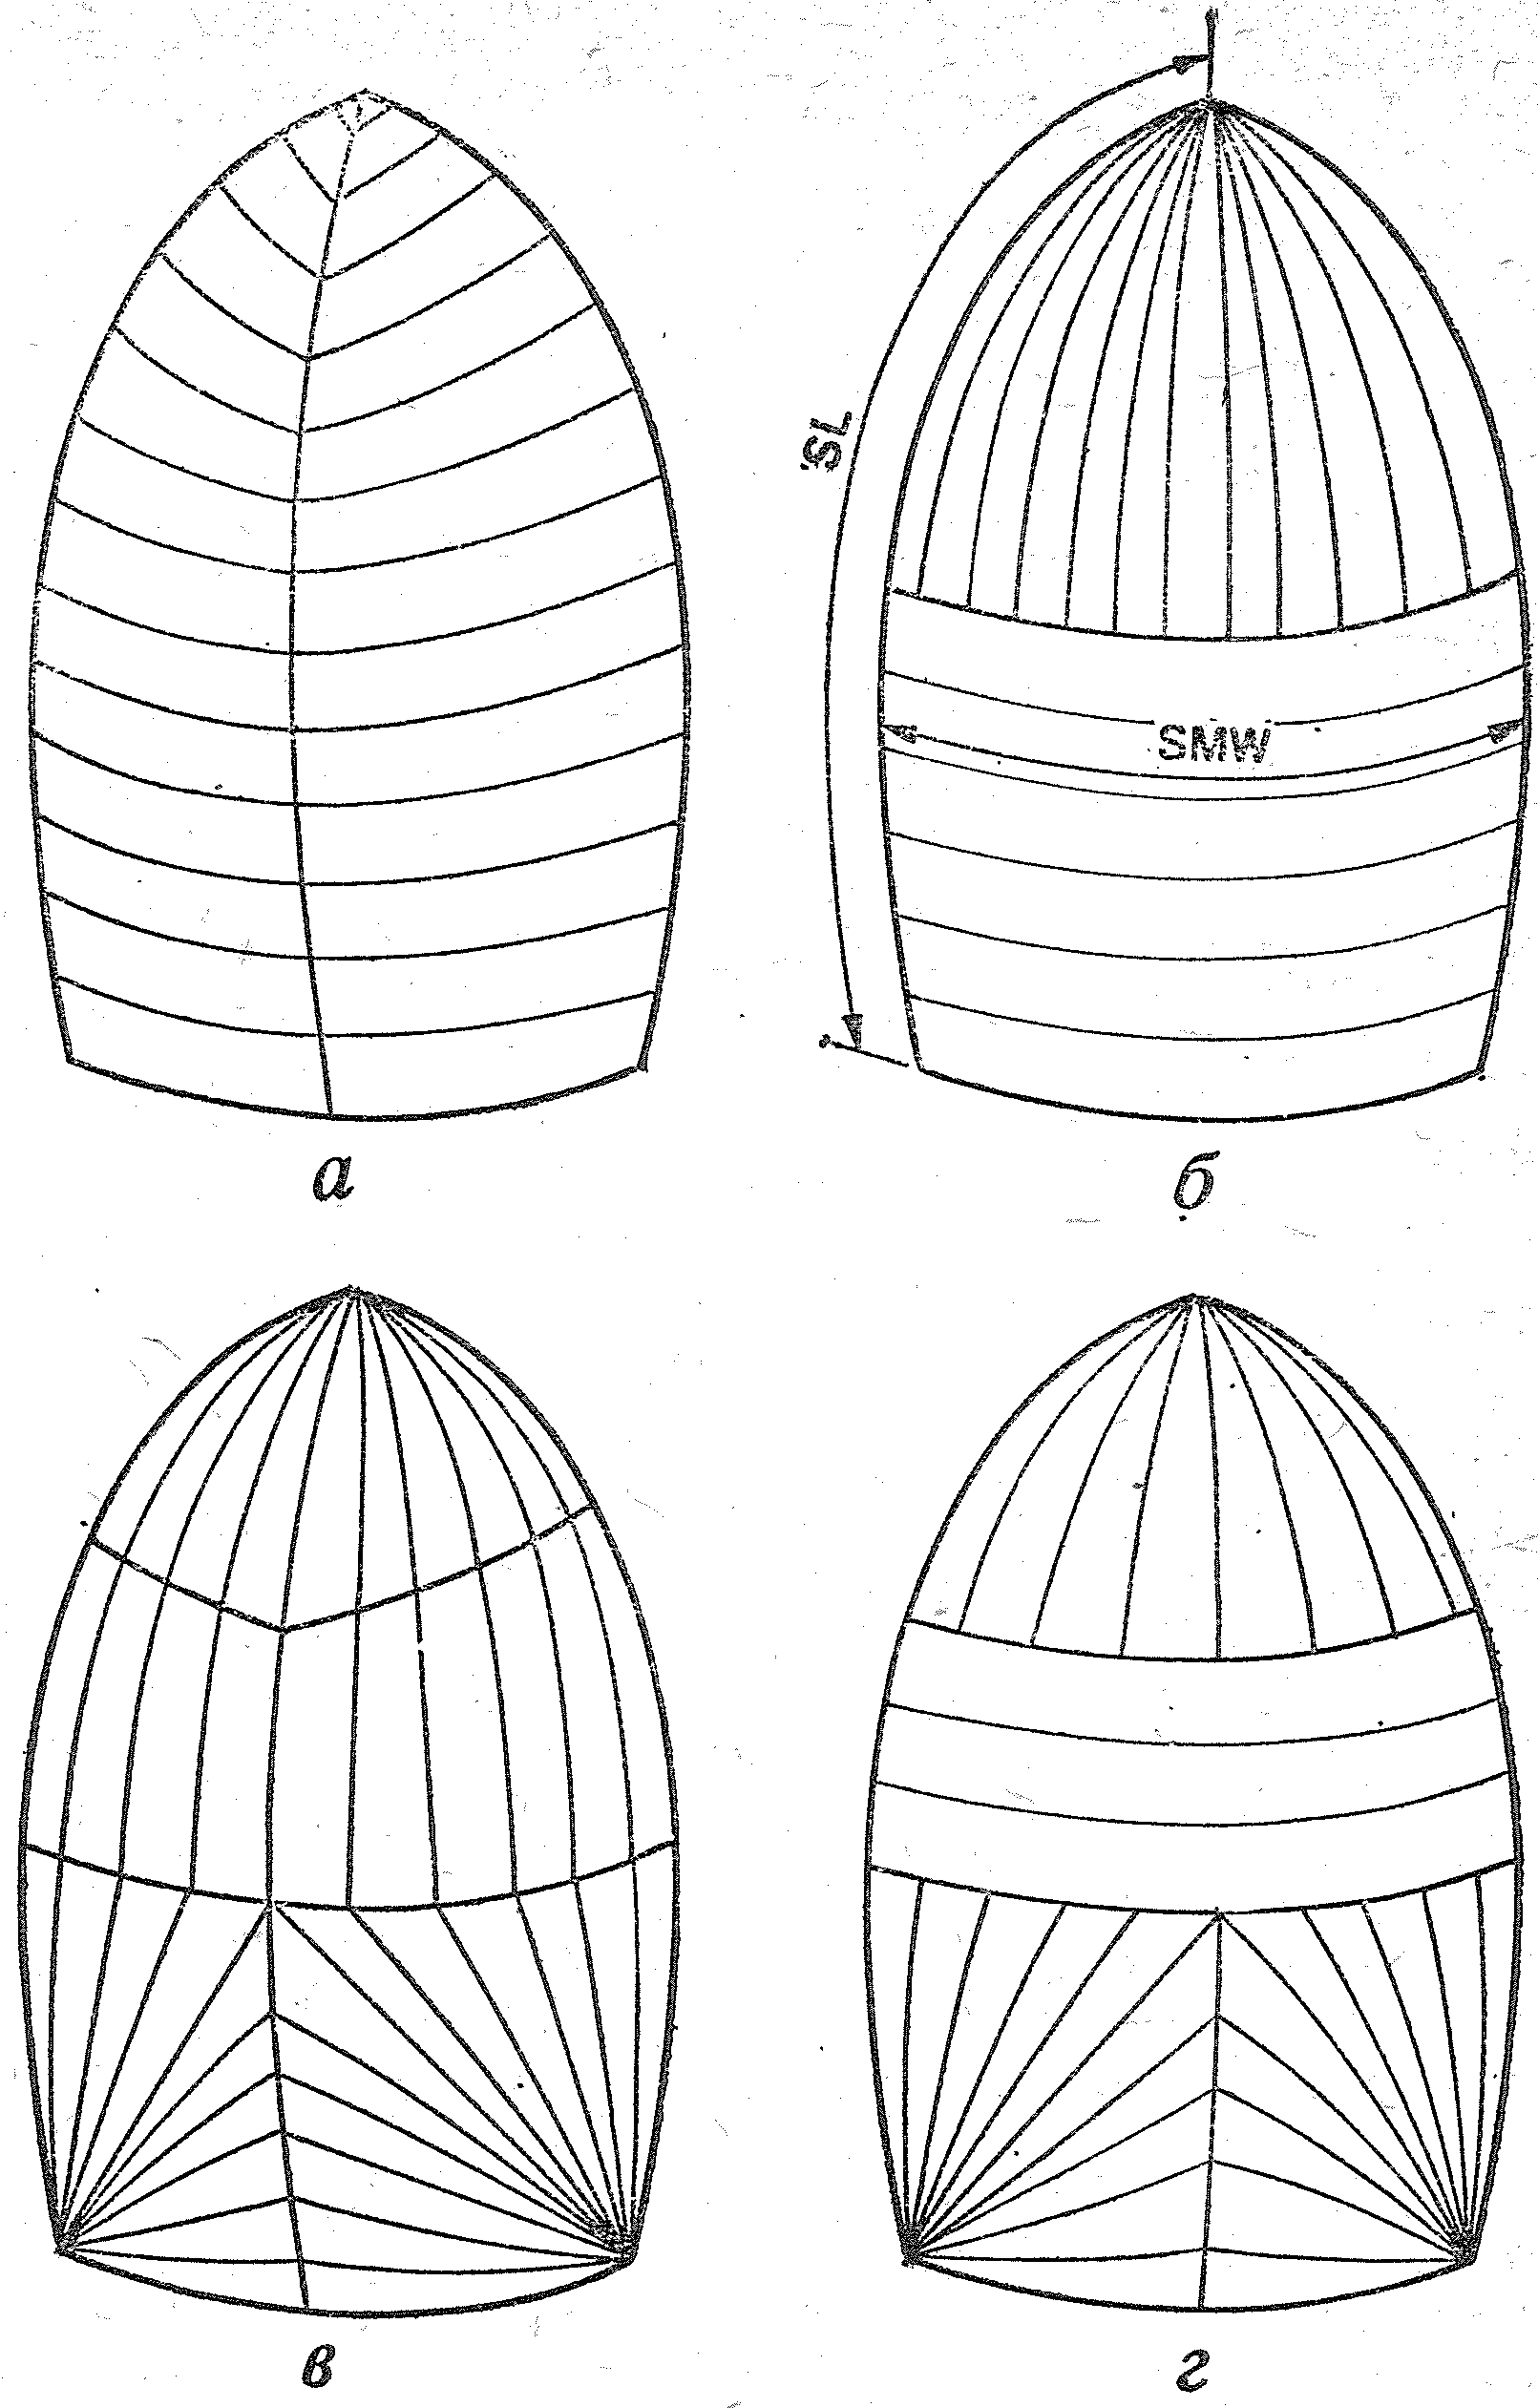
\includegraphics[scale=1.2]{0042P}
  \caption{Спинакеры}
  \label{fig:42}
  \small
  \centering{}
  Площадь сферического спинакера $S = 0,9 \cdot SL \cdot SMW$. Площадь <<звёздного>> спинакера $ S = 0,74 \cdot SL \cdot SMW$
\end{figure}

\begin{figure*}[htb]
  \centering{}
  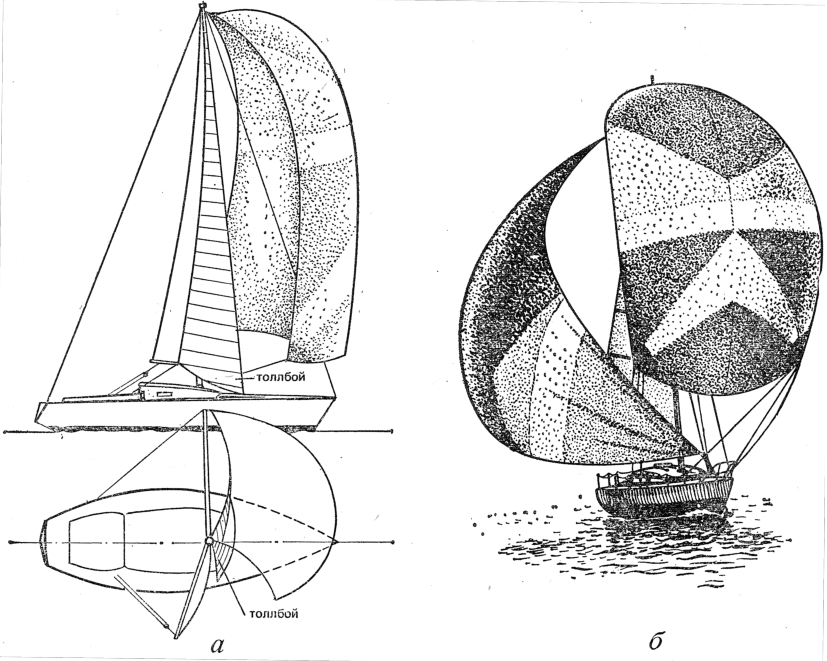
\includegraphics[scale=1.3]{0043P}
  \caption{Вспомогательные паруса для полных курсов}
  \label{fig:43}
  \small
  \centering{}
  \textit{а} \--- спинакер и толлбой; \textit{б} \--- спинакер и блупер
\end{figure*}

\begin{figure}[htb]
  \centering{}
  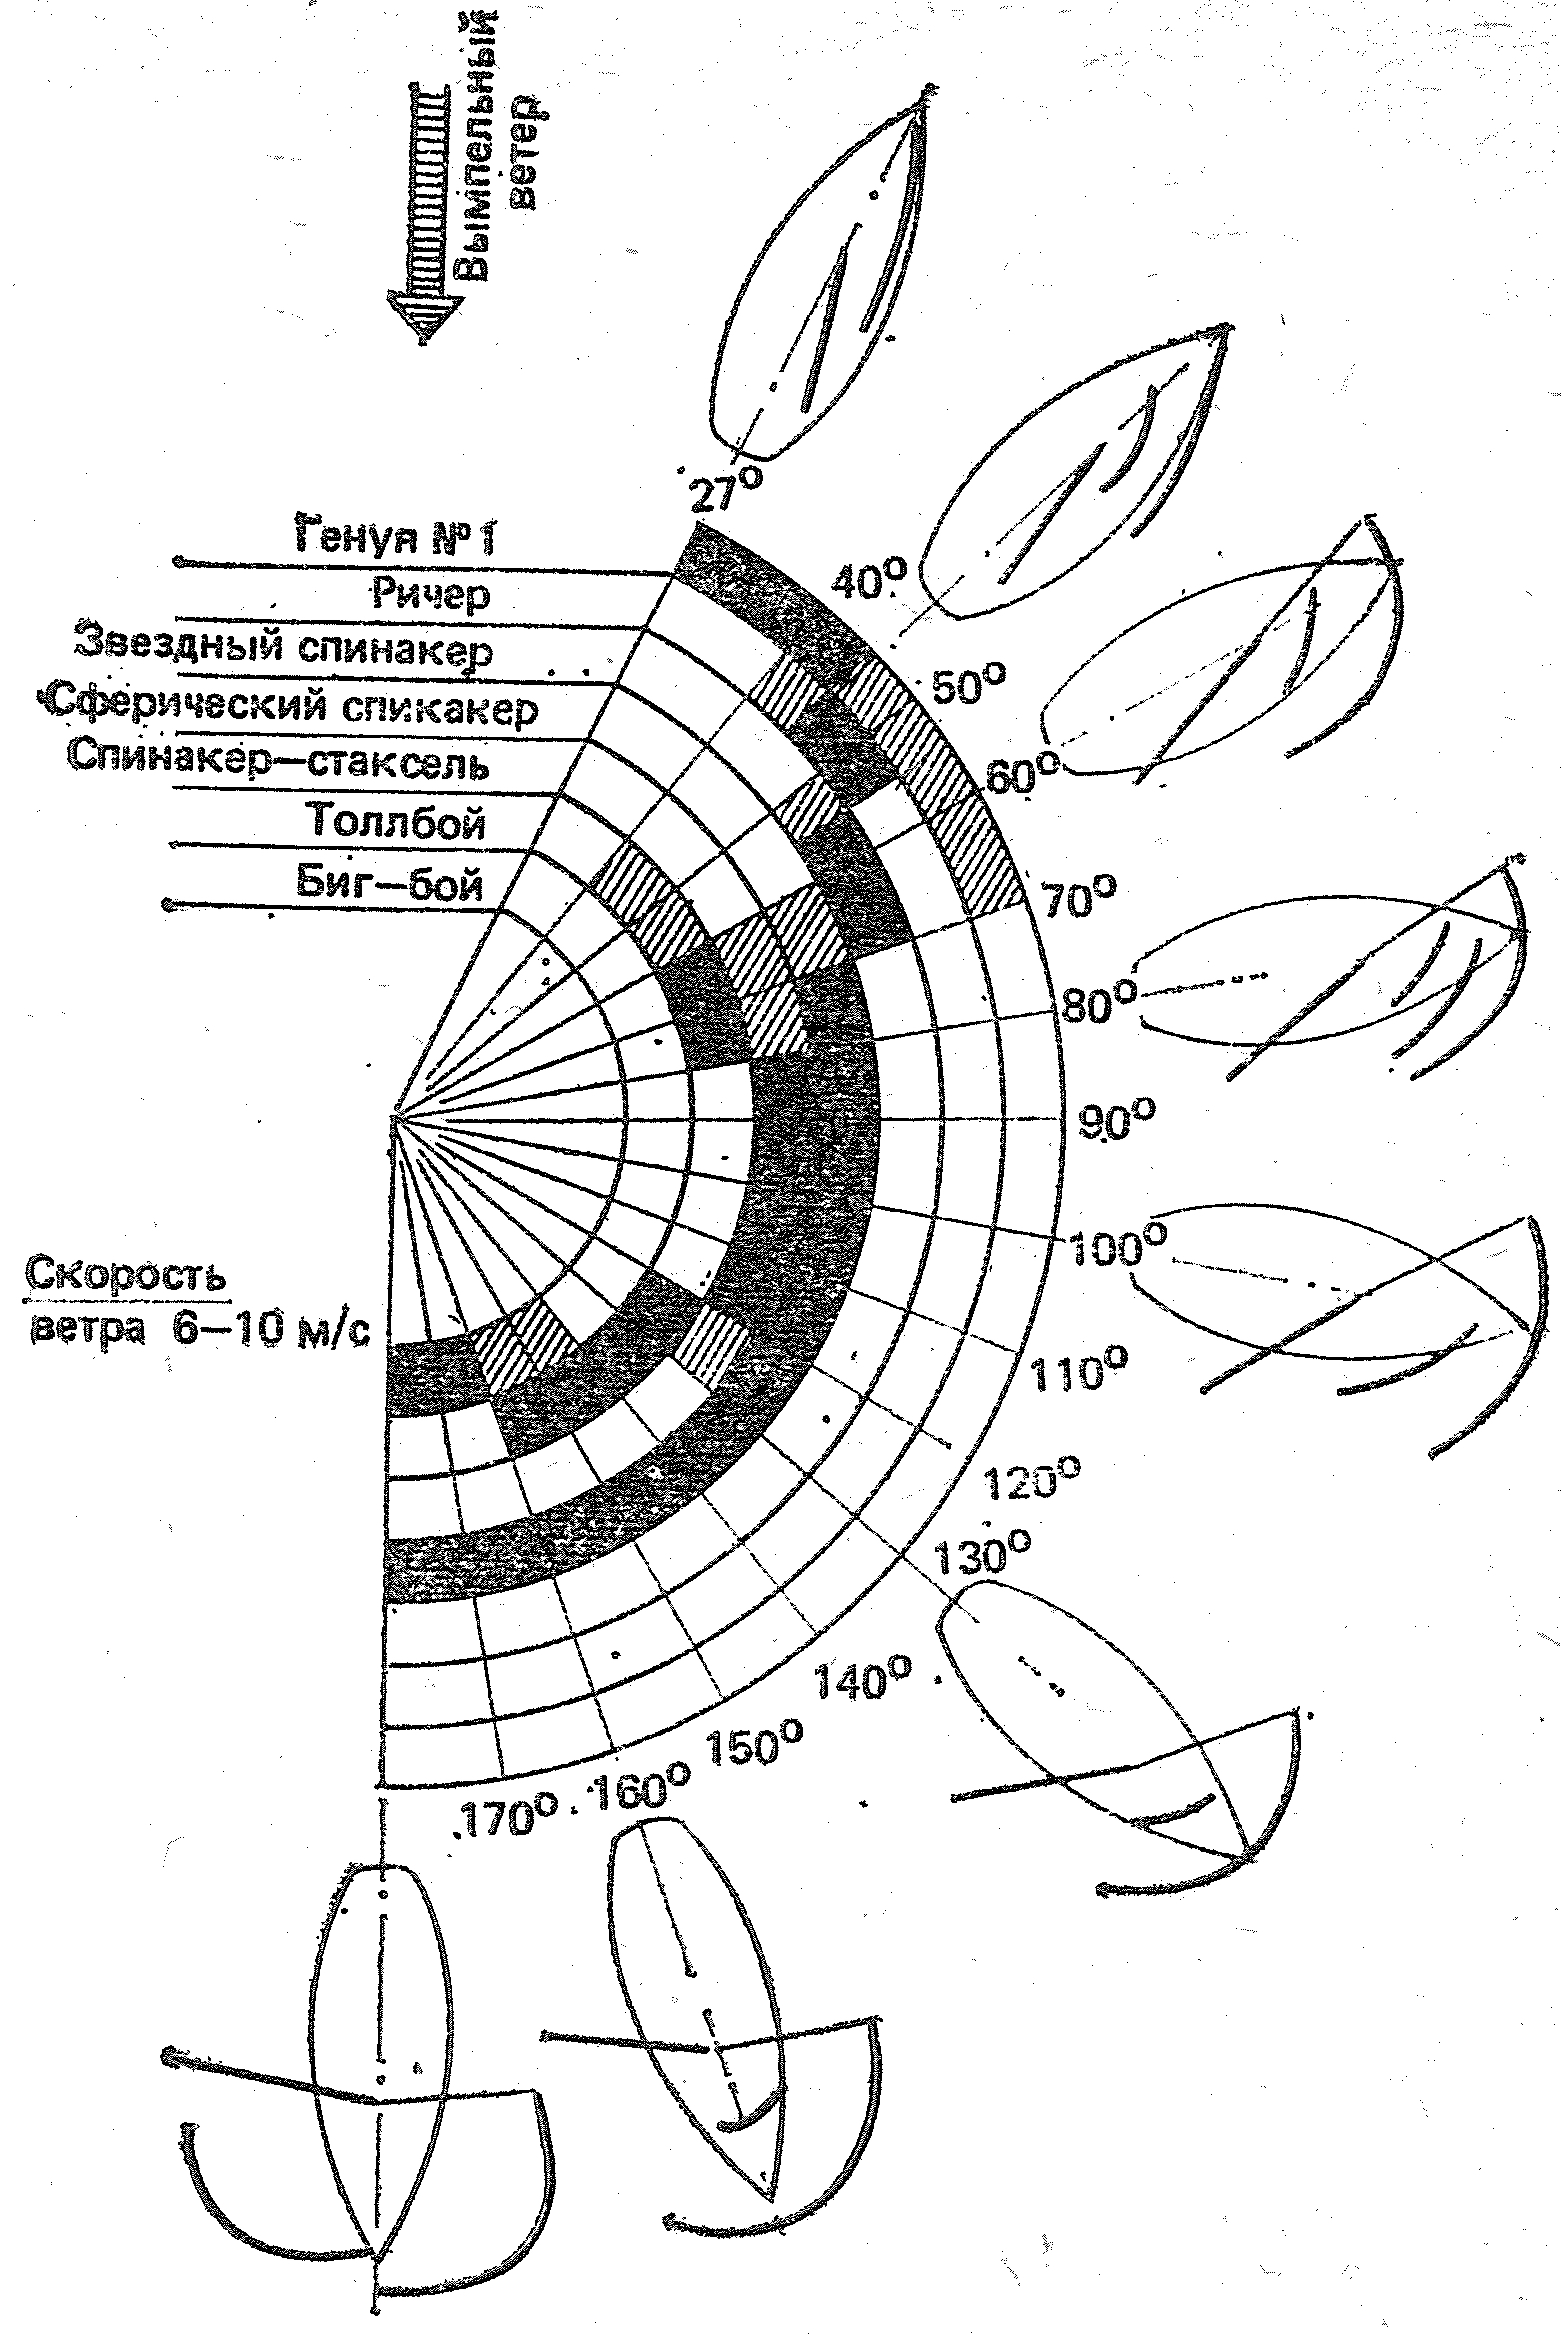
\includegraphics[scale=1.2]{0044P}
  \caption{Диаграмма применимости основных и вспомогательных парусов}
  \label{fig:44}
\end{figure}

\begin{figure*}[htb]
  \centering{}
  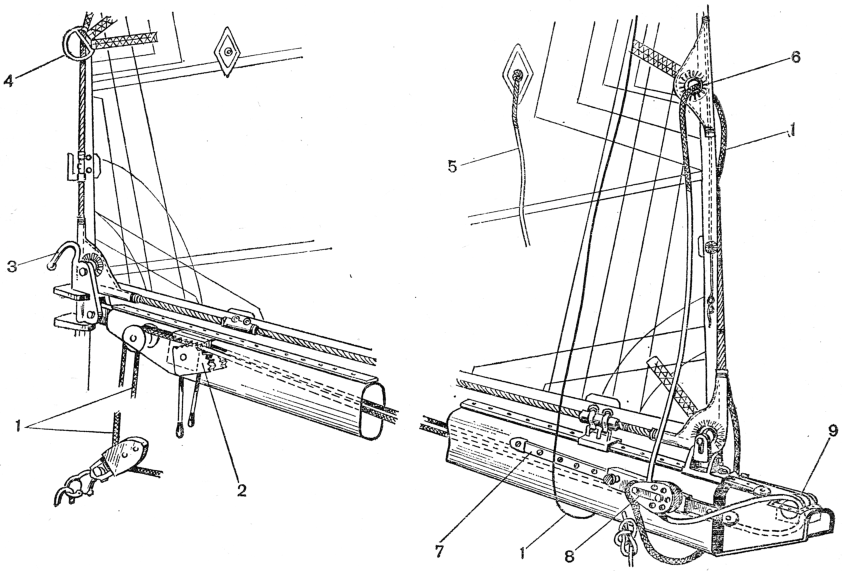
\includegraphics[scale=1.3]{0045P}
  \caption{Оснастка гика для взятия рифов}
  \label{fig:45}
  \small
  1 \--- риф-шкентели; 2 \---  стопора риф-шкентелей; 3 \--- крюк для закладывания кренгельса скобы; 4 \--- 5 \--- штерты; 6 \--- риф-кренгельс; 7 \--- рельс; 8 \--- блок риф-шкентеля на ползуне; 9 \--- врезные шкивы для шкентелей. 
\end{figure*}

\begin{figure}[htb]
  \centering{}
  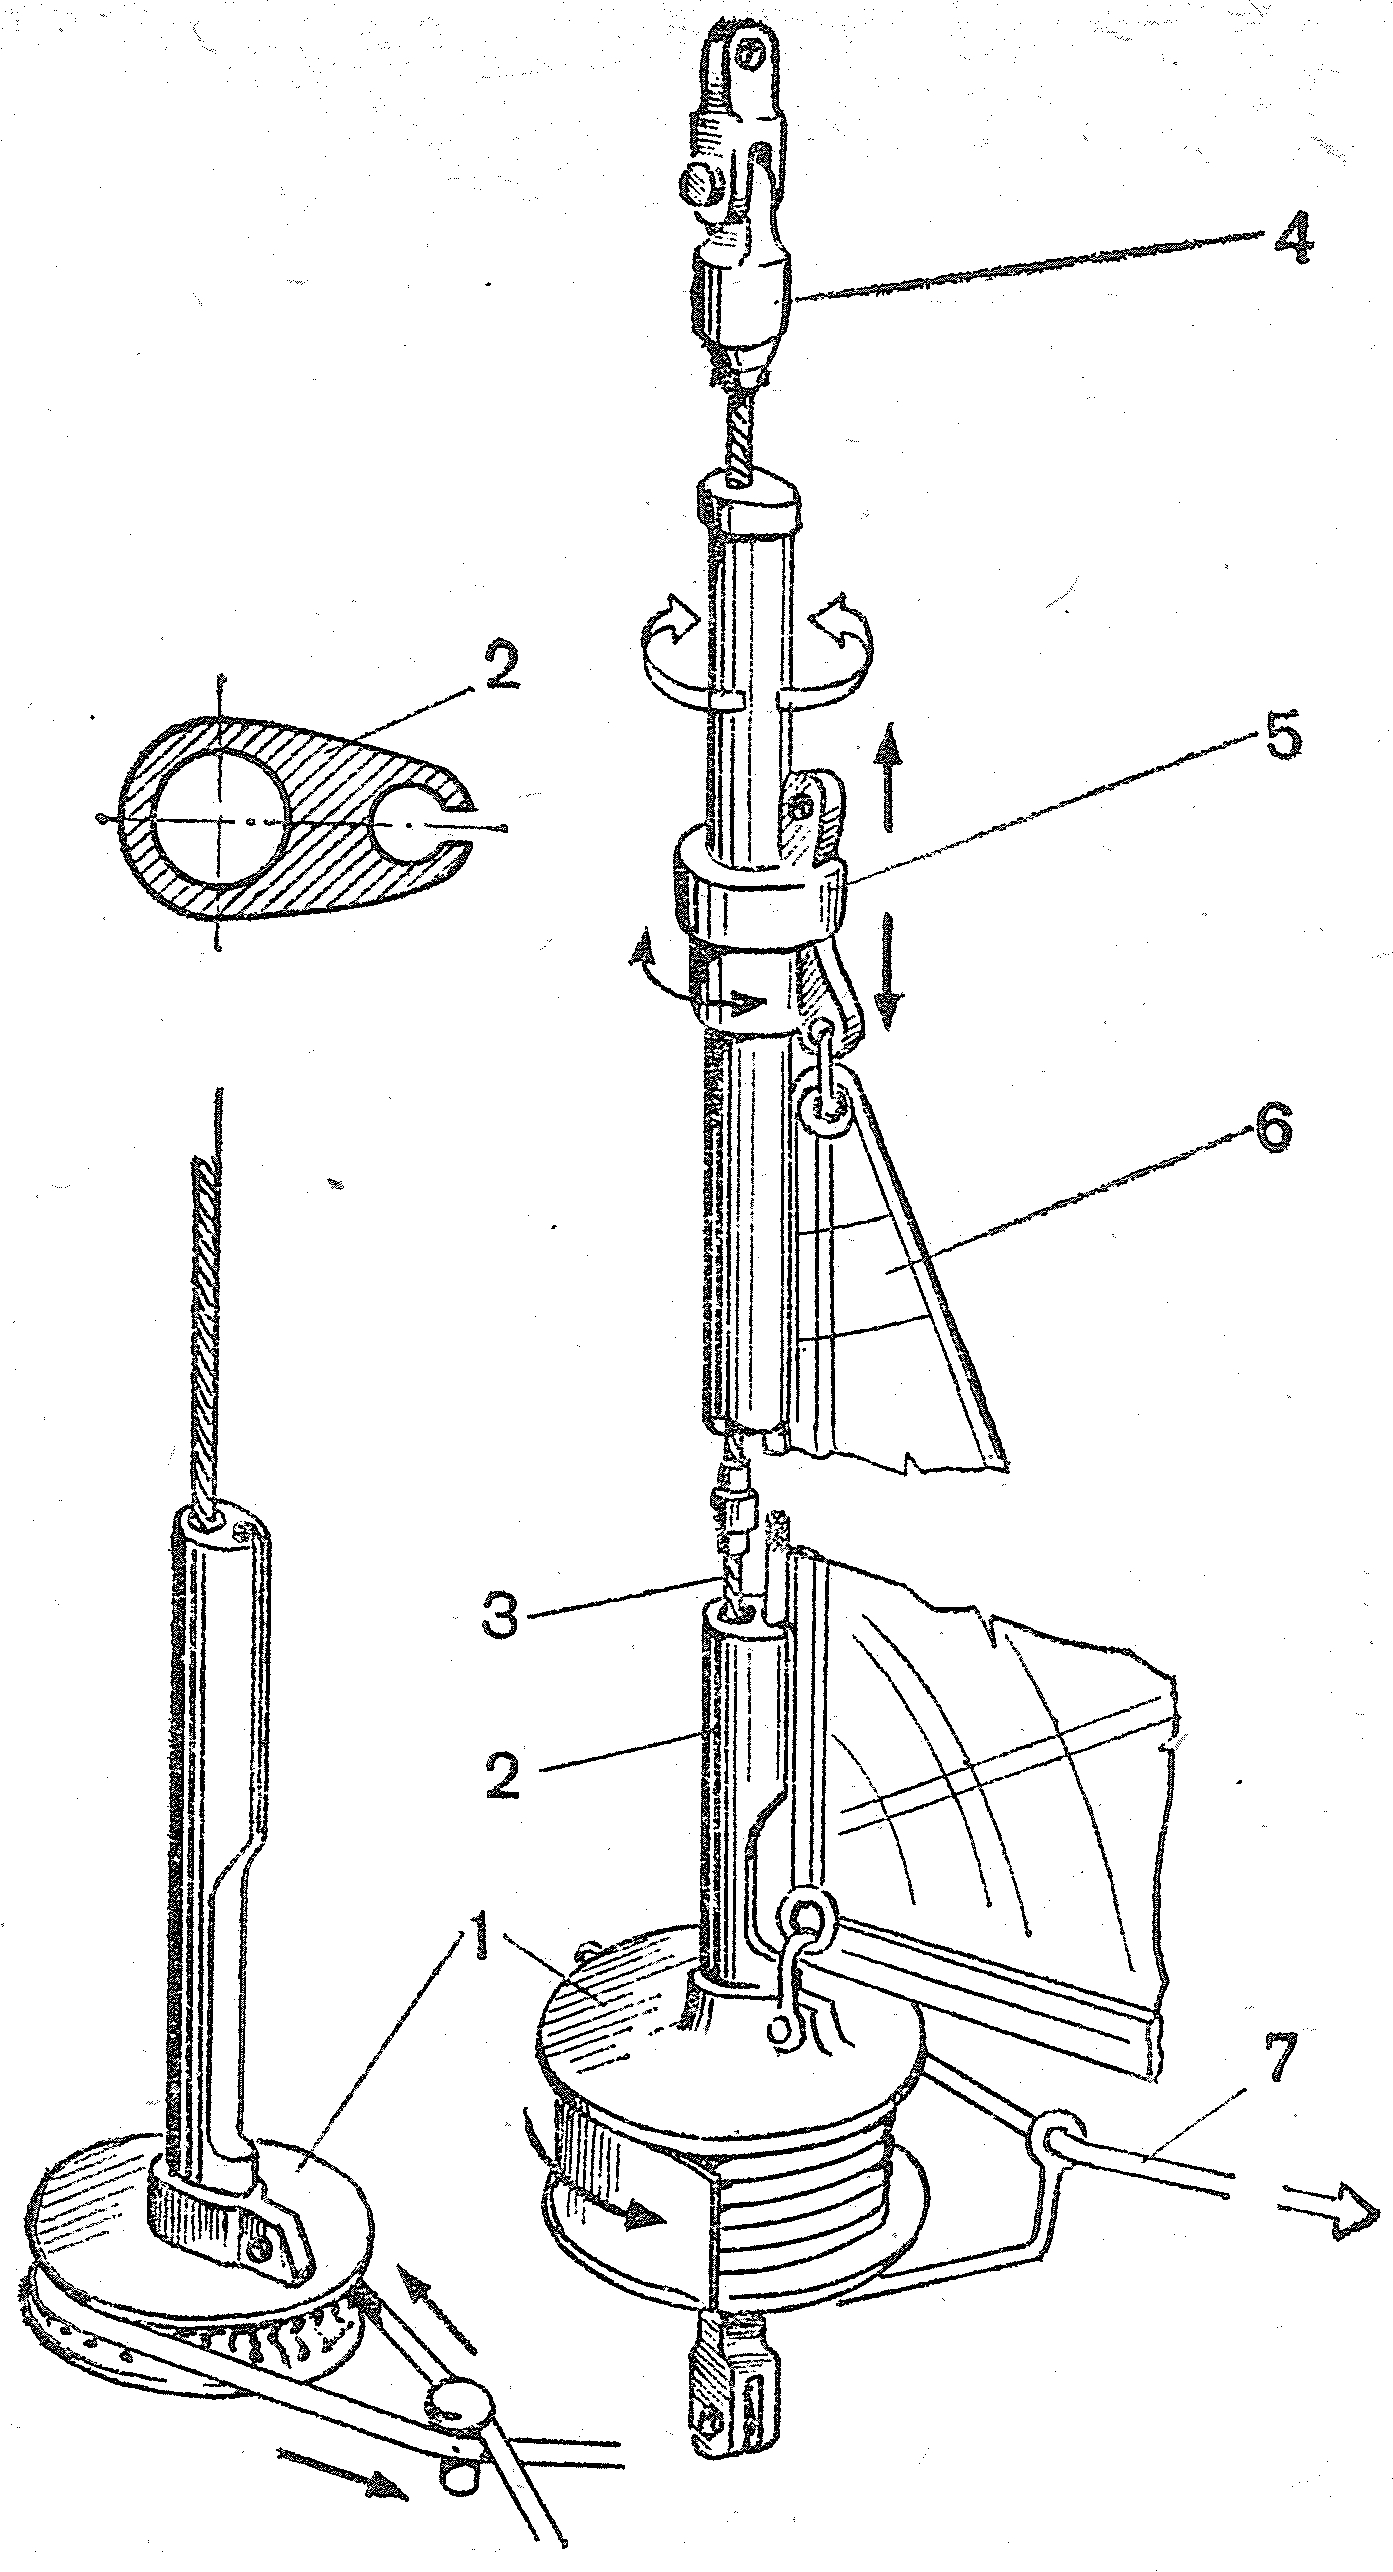
\includegraphics[scale=1.2]{0046P}
  \caption{Устройство для закрутки стакселя вокруг штага}
  \label{fig:46}
  \small
  1 \--- барабан; 2 \--- обтекатель; 3 \--- штаг; 4 \--- вертлюг; 5 \--- обойма для крепления фалового угла; 6 \--- парус; 7 \--- приводной трос
\end{figure}

При слабом ветре и на 70\gr ричер заменяют на \textbf{спинакер}\index{спинакер}\index{парус!спинакер}. В
свежий ветер (5 баллов) такая замена целесообразна уже при галфвинде,
а в сильный (6\otdo 7 баллов) \--- при крутом бакштаге.

По своей площади спинакеры являются самыми большими парусами, которые
яхта может нести при ветре данной силы. Максимальная ширина спинакера
по правилам IOR ограничивается величиной $1,8 \cdot I$, а длина
боковых шкаторин $0,95 \sqrt{I^2 + IC^2}$, где $ІC$ \--- самый больший
из следующих размеров: длина спинакер\-/гика, наибольшая ширина
спинакера, делённая на 1,8, или $I$. Существует несколько
разновидностей спинакеров, рассчитанных на разные условия плавания
(рис.\ris{42}).

\textbf{Сферический спинакер}\index{спинакер!сферический}\index{парус!спинакер!сферический}
(рис.~\ris{42}, \textit{а}) для слабого ветра шьётся из самого лёгкого
нейлона весом 30\gmsq. Выкраивается обычно из горизонтальных полотнищ,
в верхней куполообразной части может иметь средний вертикальный
шов. Для поддержания формы паруса при самых слабых дуновениях ветра
должен иметь форму верхней части, приближающуюся к полусфере. Такой
парус можно нести при ветре до 4 баллов и его курсовом угле до 60\gr.

\textbf{Радиальный спинакер}\index{спинакер!радиальный}\index{парус!спинакер!радиальный}
(рис.~\ris{42}, \textit{б}) в верхней части шьётся из полотнищ,
расходящихся лучами из фалового угла; в остальной части полотнища
горизонтальны. Покрой этого спинакера более плоский, форма купола
приближается к эллипсоиду. Материал \--- нейлон весом 50\otdo 60\gmsq;
парус рассчитан на ветер от 3 до 6 баллов при курсовых углах от 180\gr
до 60\gr.

\textbf{Спинакер <<звёздного>> покроя}\index{спинакер!звёздный}\index{парус!спинакер!звёздный}
(рис.~\ris{42}, \textit{в}) \--- очень плоский парус, предназначенный
для несения, начиная от полного бейдевинда (до 45\gr). Его площадь
превышает площадь самой большой генуи и даёт преимущество при ветре от
2 до 6 баллов. Благодаря расположению полотнищ, расходящихся из всех
трёх углов, мало деформируется под нагрузкой и не увеличивает своей
полноты при усилении ветра. Шьётся из нейлона весом до 110\gmsq с
максимально допустимой высотой, но узким. Иногда такие спинакеры
называют спанкерами.

Наконец, \textbf{штормовой спинакер}\index{спинакер!штормовой}\index{парус!спинакер!штормовой}
(рис.~\ris{42}, \textit{г}) для ветра свыше 12~м/с шьётся из нейлона
весом 110\gmsq с комбинированным или <<трирадиальным>> расположением
полотнищ: горизонтальным в средней части и лучевым в каждом углу. Это
препятствует сильному растяжению ткани, что даёт парусу излишнюю
полноту, которая приводит к образованию застойной зоны внутри
спинакера и неустойчивости его работы. Этот парус имеет площадь,
примерно равную 25\,\% площади наибольшего спинакера.

Вместе со спинакером во время гонки яхта может нести дополнительные
носовые паруса - толлбой (его назначение то же, что и в паре с генуей,
рис.~\ris{43}), блупер и подспинакерный стаксель.

\textbf{Блупер}\index{блупер}\index{шутер}\index{бигбой}\index{спинакер!подветренный}
\index{парус!блупер}\index{парус!шутер}\index{парус!бигбой}\index{парус!спинакер!подветренный}
(другие названия: шутер, бигбой, подветренный спинакер) \--- очень
полно скроенный стаксель из лёгкого нейлона весом 65\gmsq с вогнутой
передней и выпуклой нижней шкаториной, который по своим обмерам
удовлетворяет правилам IOR для стакселей и может ставиться
одновременно со спинакером на галсовой оковке для других носовых
парусов. Главный эффект блупера \--- стабилизация яхты на курсе, так
как он ставится по другую сторону от спинакера и противодействует его
уваливающему действию. Кроме того, благодаря блуперу центр парусности
перемещается вперёд, умеряется раскачивание яхты, фаловый угол блупера
\--- свободный, и фал служит таким же инструментом для управления
парусом, как шкот и брас для спинакера. Блупер ставится при ветре от 3
до 13~м/с на курсах от полного бакштага до чистого фордевинда
(160\otdo 180\gr).
 
Поскольку грот создаёт помехи для устойчивой работы спинакера и
блупера, в свежий ветер и при спокойном море на нем берут риф, а в
слабый ветер его лучше убрать совсем.

При направлении ветра к курсу яхты под углом 135\gr и менее нести,
блупер становится нецелесообразно и его заменяют толлбоем или
подспинакерным стакселем.
 
Диаграмма, приведённая на рис.~\ris{44}, суммирует сказанное о
применимости различных носовых парусов в средний ветер в зависимости
от курса яхты относительно ветра. Залитые чёрным сектора обозначают
рекомендуемый диапазон для несения паруса, заштрихованные \---
возможный.

Кроме основных и дополнительных парусов каждая яхта, участвующая в
крейсерских гонках должна снабжаться штормовыми парусами \---
стакселем и триселем.

\textbf{Бегучий такелаж.}\index{бегучий такелаж}\index{такелаж!бегучий}
Фалы парусов вырубают из гибких
стальных тросов двойной свивки, изготовленных из нержавеющей или
оцинкованной стальной проволоки. Используются тросы конструкции
$7 \times 19$, состоящие из шести прядей по 19 проволок в каждой и
такой же седьмой, служащей центральным сердечником, или
$6 \times 19 + $\,ос \--- с сердечником из растительной пряди. Для
надёжности и долговечности фала важно, чтобы он имел достаточный запас
прочности (не менее 4 и не менее 6 в тех случаях, если фал может быть
использован для подъёма человека на мачту) и был проведён через шкивы
достаточно большого диаметра. Если трос огибает шкив под углом 180\gr,
то диаметр шкива (по желобку для троса) не должен быть менее 20
диаметров троса. Если же направление тяги троса изменяется на 90\gr,
то критическим будет диаметр шкива, равный 16 диаметрам троса. Огибая
шкивы меньшего диаметра, проволоки троса подвергаются большим
напряжениям снятия, и при повторяющихся на качке перемещениях фала по
шкиву трос быстро изнашивается. Также важно, чтобы шкивы были
изготовлены из более мягкого, чем сталь, материала \--- прочной
пластмассы или бронзы.

На топ мачты обычно проводится один грота\-/фал, два фала генуи и два
спинакер\-/фала (обычно с вертлюжным блоком). Кроме того, на мачте
может быть фал для стакселя, топенанта грота- и спинакер-гиков. При
металлической мачте фалы проводятся внутри неё таким образом, чтобы
исключалось переплетение отдельных тросов между собой. В нижней части
мачты фалы выводят наружу и через направляющие футблоки проводят на
лебёдки шпилевого типа, обычно устанавливаемые впереди кокпита
команды.

Гика\-/шкот проводится даже крупных яхтах в 4 лопаря \--- необходимое
усилие для добирания обеспечивается специальной лебёдкой. Вместо
двухшкивных предпочтительнее одинарные блоки, при которых трос не
закручивается и легко травится без его раздергивания. Нижние блоки
крепят к ползуну, перемещаемому по поперечному погону с помощью
специальных талей.

Для генуи часто применяют шкоты из стального троса, наращивая их на
ходовых концах короткими отрезками синтетического троса для
закладывания на барабан лебёдки. Такие комбинированные шкоты хороши
тем, что не вытягиваются в сильный ветер и позволяют сохранить угол
атаки паруса при порывах ветра. Для спинакер\-/шкотов хорош
полипропиленовый трос, который не намокает, а спинакер\-/брас лучше
вырубить из стального тросика \--- он не вытягивается и позволяет
сохранить оптимальную настройку спинакера при порывах ветра.

Оттяжка гика в виде многократных талей на новейших яхтах заменяется
винтовым или гидравлическим талрепом, что позволяет отказаться от
проводки гика\-/топенанта.

На рис.~\ris{45} представлена проводка бегучего такелажа для взятия
рифов на гроте, а на рис.~\ris{46} \--- схема устройства для закрутки
стакселя вокруг штага, снабжённого обтекателем с ликпазом. На гоночных
яхтах это устройство используется для временной уборки генуи при
замене её спинакером либо другим парусом, имеющим свободную переднюю
шкаторину. Удобен также обтекатель штага с двумя ликпазами, который
позволяет в спокойной обстановке поставить новый стаксель, а затем
убрать предыдущий.

В крейсерском плавании устройство для закрутки стакселя может быть
использовано для уменьшения его площади, особенно если он скроен
специально для этой цели плоским и с высоким шкотовым углом. Последнее
позволяет при закрутке стакселя использовать одни и те же кипы
стаксель\-/шкотов.

%%% Local Variables:
%%% mode: latex
%%% TeX-master: "yacht-captain"
%%% End:
